\begin{quotation}
  {\footnotesize
    \noindent{\emph{``Most good programmers do programming not because they expect to get paid or get adulation by the public, but because it is fun to program.''\\}
    }
    \begin{flushright}
      Linus Torvalds
    \end{flushright}
  }
\end{quotation}
\vspace{0.5cm}

In this chapter the reader will first be presented with a qualitative analysis of the images produced with the toolbox illustrated in chapter \ref{chap:second-chapter}. After that, the preliminary validation of the \acrshort{svd} algorithm presented in chapter \ref{chap:third-chapter}  when applied to the same images will be discussed.

\section{Qualitative Assessment}
The aim of the toolbox presented in chapter \ref{chap:second-chapter} was to create batches of realistic images of a given CAD of a \acrshort{sc} in order to cope with the lack of an actual facility to produce images from a scale \acrshort{3d} printed model of the target itself, as done in \cite{Beierle2019}. Validating the goodness of the generated images is extremely difficult because of the actual lack of high-resolution and high-quality images taken in orbit by a real camera of a real \acrshort{sc}. So, the more realistic intent of this evaluation is therefore to compare the generated images to the images found in the SPEED data-set \footnote{The SPEED data-set is freely available at \url{https://kelvins.esa.int/satellite-pose-estimation-challenge/}}, in order to identify similarities and differences. As proposed in \cite{pangufinal}, the images can be compared in three ways:

\begin{itemize}
  \item visual comparison;
  \item image histogram comparison;
  \item basic feature extraction using a Sobel edge detector.
\end{itemize}

Unfortunately, the orbit and the true pose but more importantly the illumination conditions of each of the images contained in the SPEED data-set was not available at the time of writing this thesis, so it is impossible to present to the reader a one-to-one comparison. Still, it is worth to compare images which can be reasonably considered similar.

\begin{figure}[htbp]
  \centering
  \includegraphics[width=1.0\textwidth]{gfx/comparison/comparison1.eps}
  \caption{Comparison between the SPEED data-set (left) and images generated using the toolbox presented in chapter \ref{chap:second-chapter} (right), 1}
  \label{fig:comparison1}
\end{figure}

\begin{figure}[htbp]
  \centering
  \includegraphics[width=1.0\textwidth]{gfx/comparison/comparison2.eps}
  \caption{Comparison between the SPEED data-set (left) and images generated using the toolbox presented in chapter \ref{chap:second-chapter} (right), 2}
  \label{fig:comparison2}
\end{figure}

\begin{figure}[htbp]
  \centering
  \includegraphics[width=1.0\textwidth]{gfx/comparison/comparison3.eps}
  \caption{Comparison between the SPEED data-set (left) and images generated using the toolbox presented in chapter \ref{chap:second-chapter} (right), 3}
  \label{fig:comparison3}
\end{figure}

\begin{figure}[htbp]
  \centering
  \includegraphics[width=1.0\textwidth]{gfx/comparison/comparison4.eps}
  \caption{Comparison between the SPEED data-set (left) and images generated using the toolbox presented in chapter \ref{chap:second-chapter} (right), 4}
  \label{fig:comparison4}
\end{figure}

In figures \ref{fig:comparison1}, \ref{fig:comparison2}, \ref{fig:comparison3} are presented three simulated images of the Tango \acrshort{sc} on a black background.
Overall, it is possible to recognize that the images belonging to the SPEED shows a better representation of the external look of the \acrshort{sc}, for both the solar panels and the external appendages and external structures. Usually, for rendering images of \acrshort{sc}s, the manufacturer makes available textures of the external look of the whole \acrshort{sc}. For this project unfortunately, due to the unavailability of said textures, the whole look of had to be recreated by hand, doing several experiments and comparisons. This is particularly visible when looking at solar panels, where the SPEED images are of an order of magnitude superior in terms of accuracy and realness of what is being represented.
Despite said issues however, by looking at the forms of the histograms it is possible to recognize that histograms belonging to the SPEED images and histograms belonging to the images used though this project are essentially similar. They both shows the same exponential behavior. The images belonging to the SPEED data-set shows an overall greater concentration of dark values with respect to the ones generated with the toolbox presented in chapter \ref{chap:second-chapter}. This is likely to be due to slightly different scenes being represented in terms of illumination conditions and shadows.
The Sobel edge images are also very similar. The images generated for this project presents a slightly higher level of noise (recognizable by the more presence of little white pixels). This can be due to a different $\sigma^2$ value used to add Gaussian white noise to the image during the post-processing phase.
Lastly, in figure \ref{fig:comparison4} is showed a comparison were the Earth is in the background. As it can be clearly seen by the reader, the Earth is represented more accurately in the SPEED data-set, but this is simply due to the fact that for the SPEED data-set the Earth images comes from actually real space imagery. As described in \cite{Sharma2019}, the Earth images used for the SPEED data-set are composed by 72 actual images of the Earth captured by the Himawari-8 geostationary meteorological satellite. The 72 images each provide a \num{100e6} pixels resolution disk-view of the Earth and were taken 10 minutes apart from each other over a period of 12 hours. The quality the Earth has in the images generated with the toolbox developed during this work can be enhanced by using a texture with an higher resolution, however this comes at the cost of long rendering times and greater RAM usage for rendering the single image. Generating one single image where the Earth is present in the background takes approximately \SI{3}{\s} and occupy \textit{circa} $2$ Gb of RAM on an Intel Core i7-4500U CPU when using mercator images rescaled to $21600 \times 10800$ pixel resolution. Better results can be archived using the full $43200 \times 21600$ pixel original mercator images but rendering times as well as RAM usage would grow too much for the generation of a data-set of hundreds of images on the previously mentioned H/W.

\section{\acrshort{svd} architecture tests}
A further validation of the generated data-set can be obtained by analyzing the synthetic images using a \acrshort{cv} algorithm. In fact, if the quality of the generated images is poor, where for poor it is intended not being photorealistic, the \acrshort{cv} algorithm will not work consistently. Among all state-of-the-art \acrshort{cv} algorithms available, the \acrshort{svd} algorithm has been selected because of its simplicity and effectiveness.
The identification of a correct \acrshort{roi} is of vital importance since the edge detection process as well as the merging edges block depends on geometrical parameters which are set as multiplicative constants of the diagonal length of the \acrshort{roi}. From a first batch of tests realized using the images generated using the toolbox presented in chapter \ref{chap:second-chapter}, the \acrshort{roi} detection performances of the \acrshort{wge} technique are consistent with what found in \cite{Sharma2018} and \cite{fracchio2019}. When the image has a black or nearly black background, the results of the \acrshort{wge} are very good, and in almost all cases it's capable of identifying the correct \acrshort{roi}. However, the presence of a composite background (such as the Earth) in some cases negatively affects the performances of the \acrshort{wge} technique. This is due to the fact that the presence of the Earth produces spurious element in the gradient image, which are not eliminated by the filtering procedure. This particular behavior can be observed for example in figures \ref{fig:roiResults1}a, \ref{fig:roiResults1}h and \ref{fig:roiResults2}e.

\begin{figure}[htbp]
  \centering
  \subfloat[]{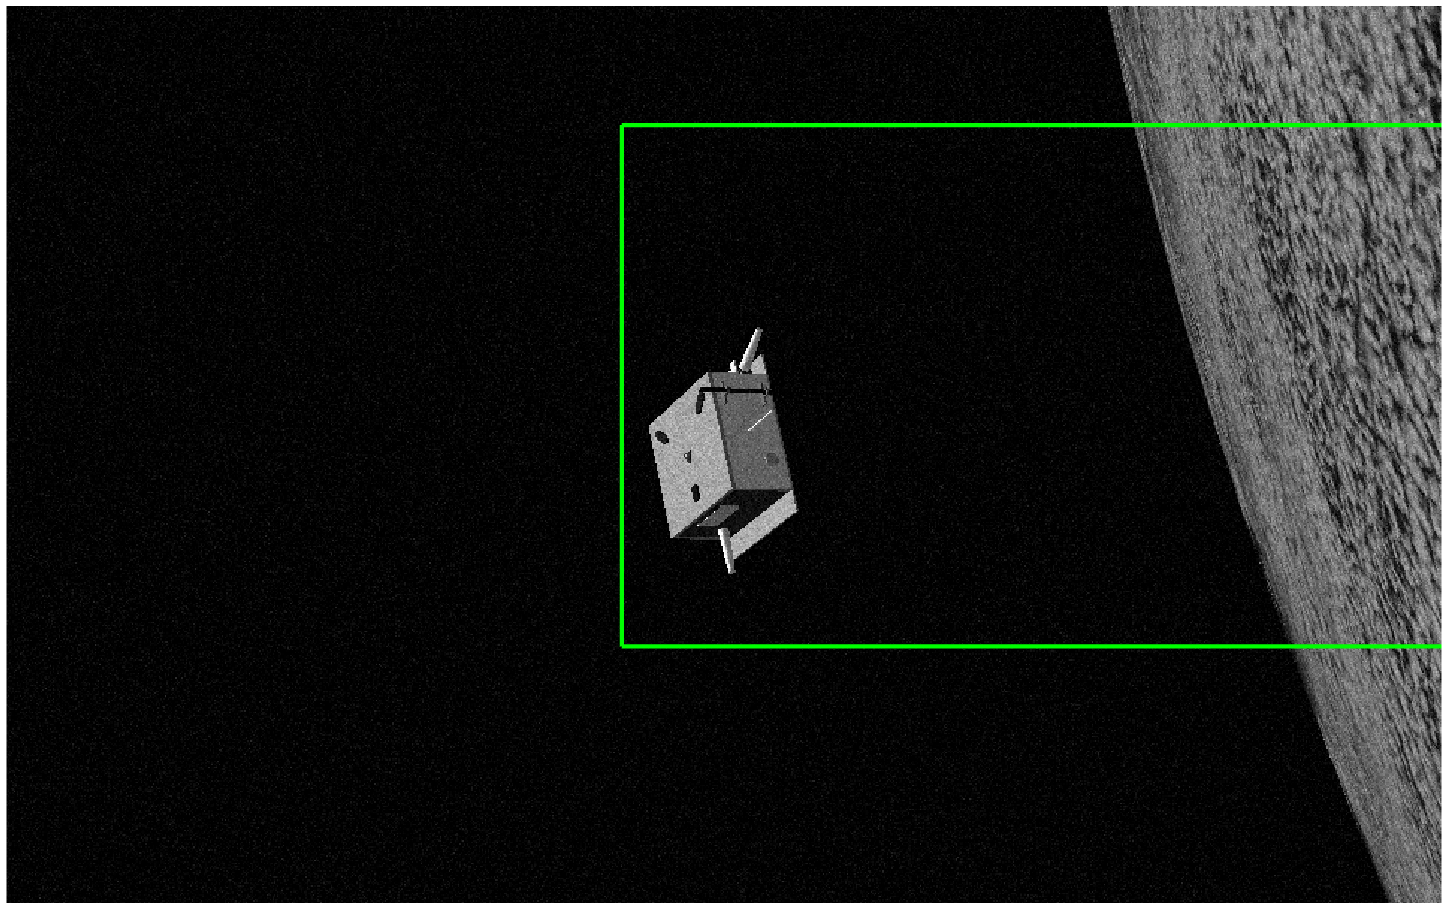
\includegraphics[width=0.45\textwidth]{gfx/results/prisma/101/9.png}}
  \qquad
  \subfloat[]{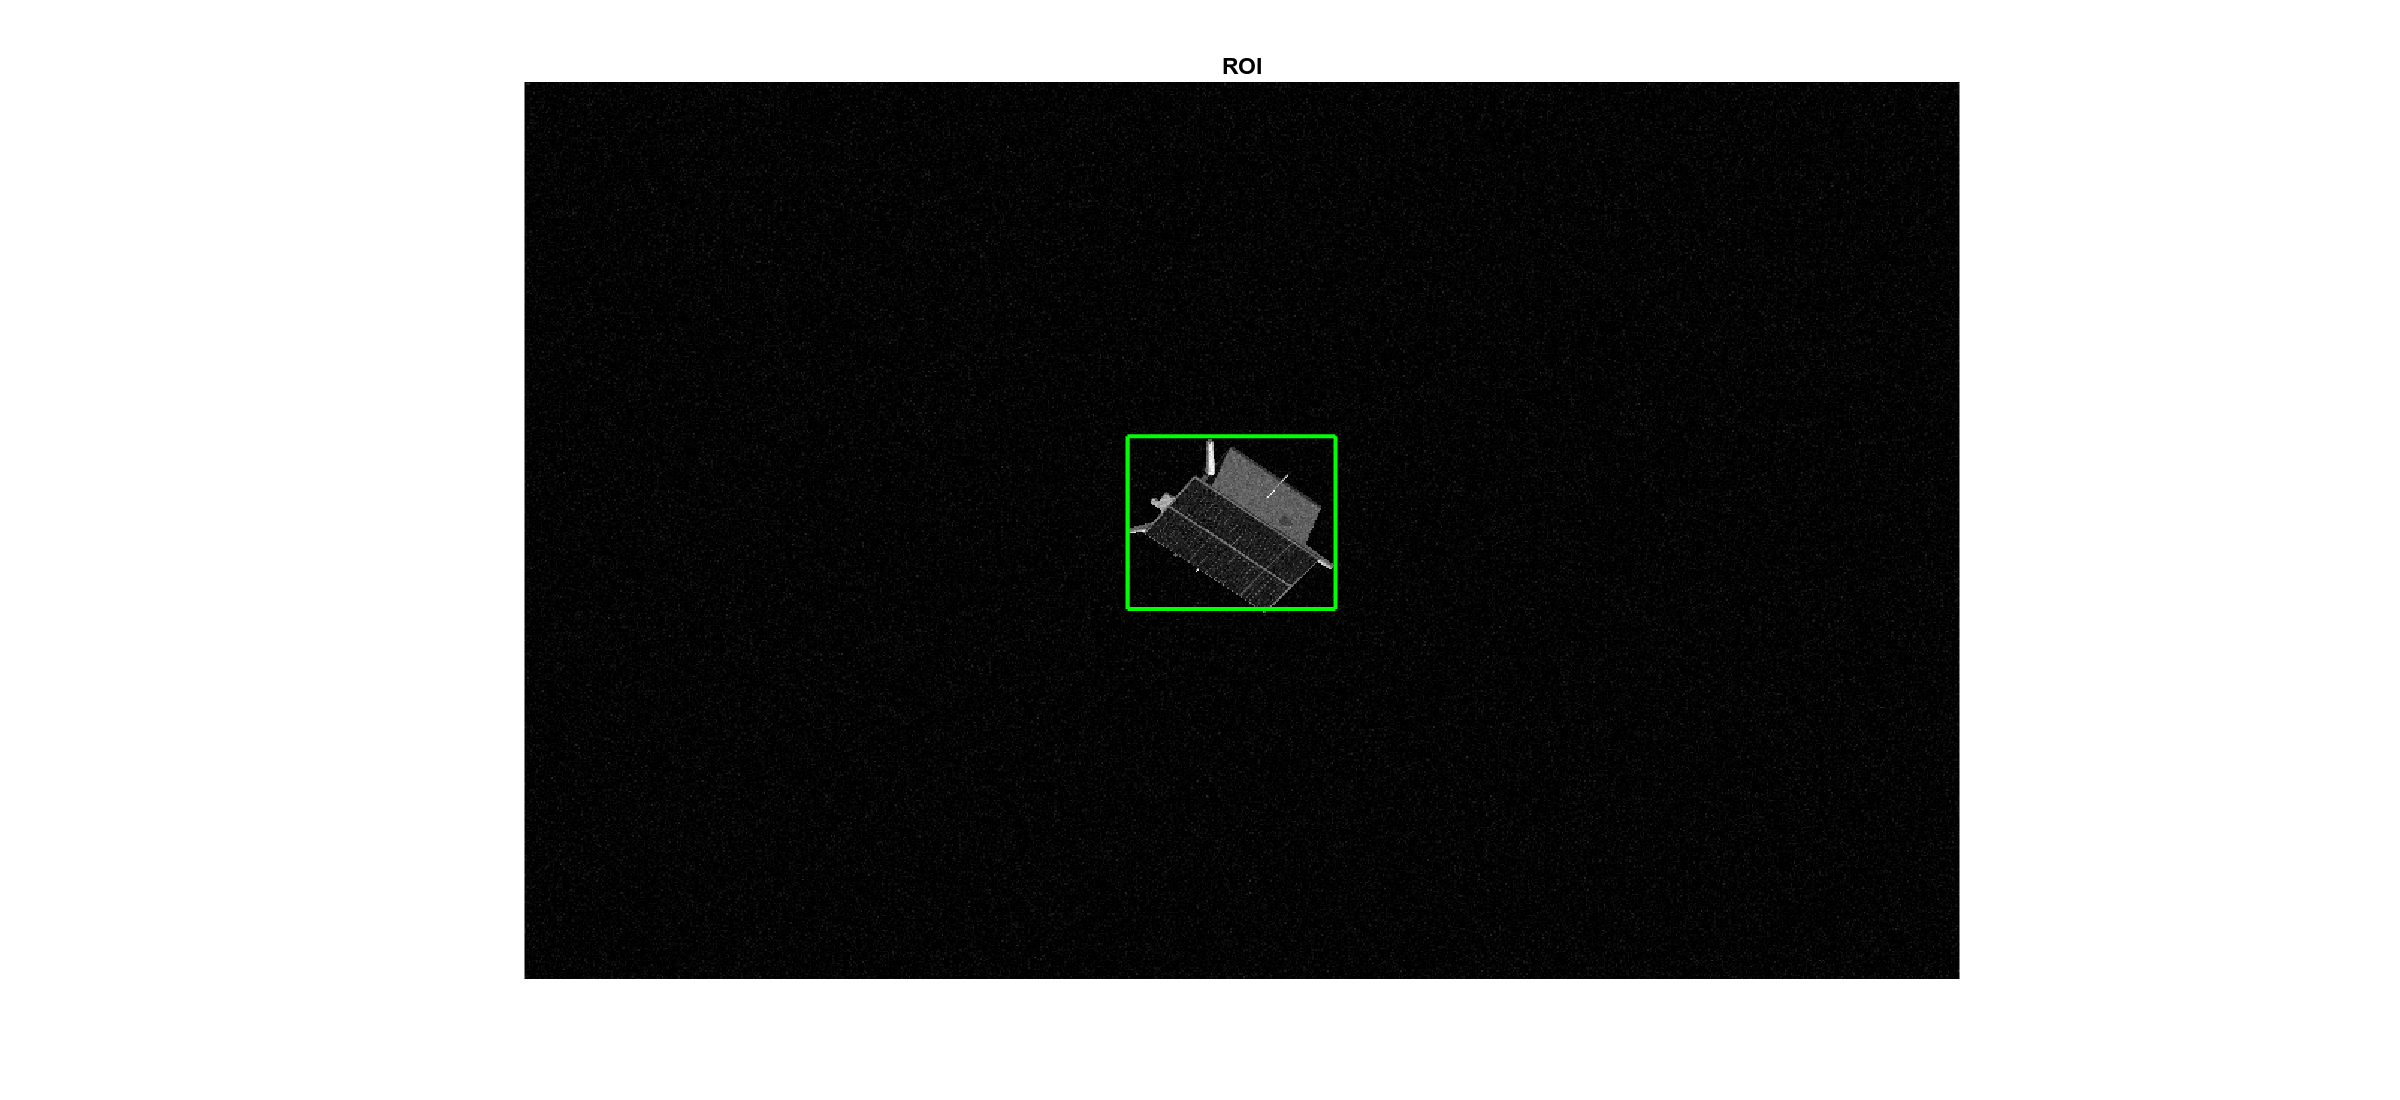
\includegraphics[width=0.45\textwidth]{gfx/results/prisma/111/9.png}}
  \qquad
  \subfloat[]{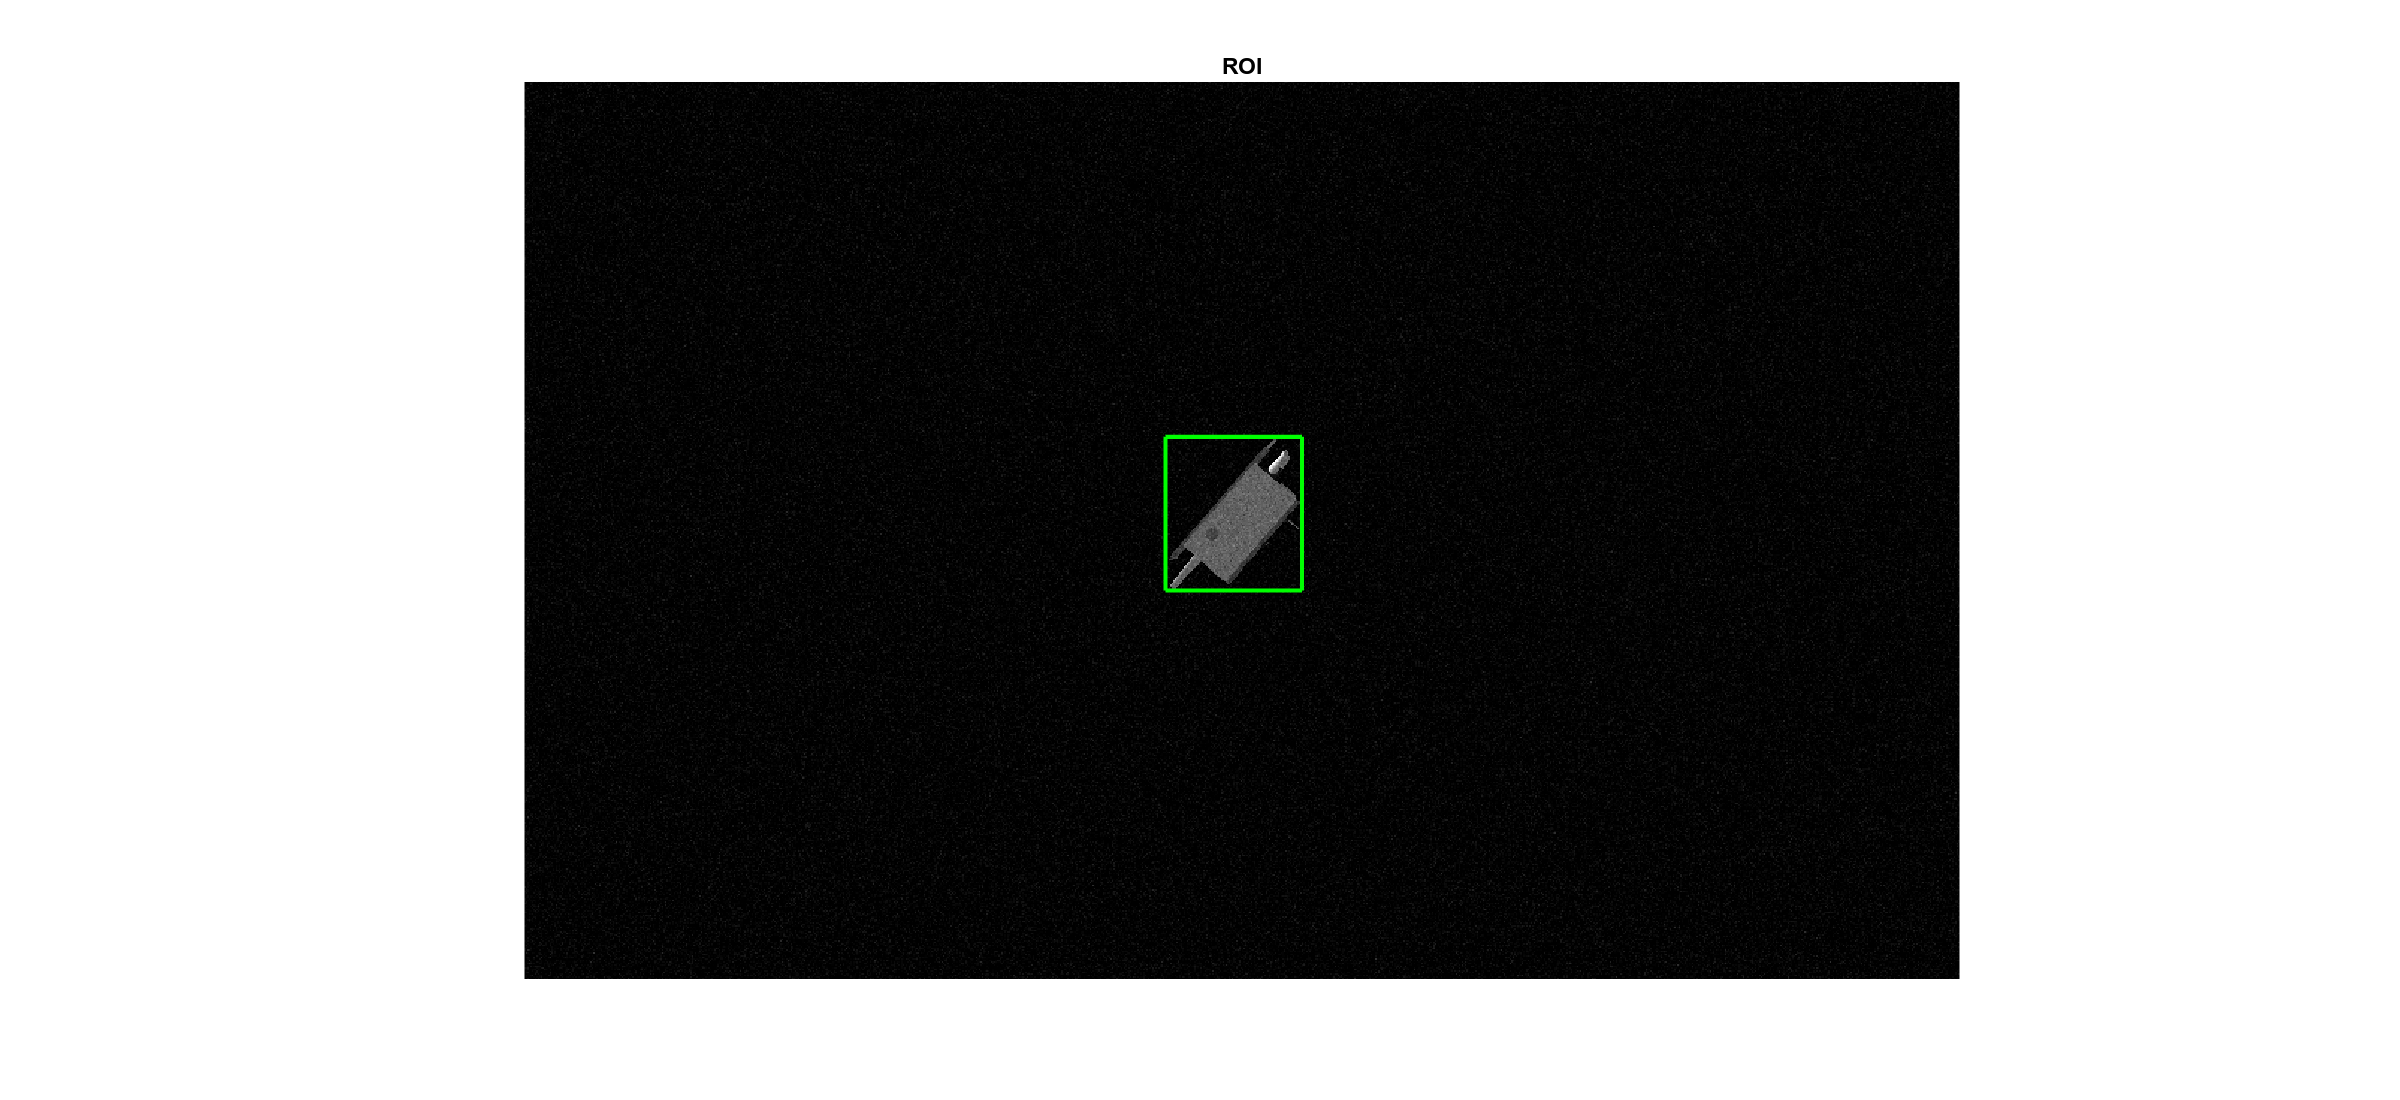
\includegraphics[width=0.45\textwidth]{gfx/results/prisma/112/9.png}}
  \qquad
  \subfloat[]{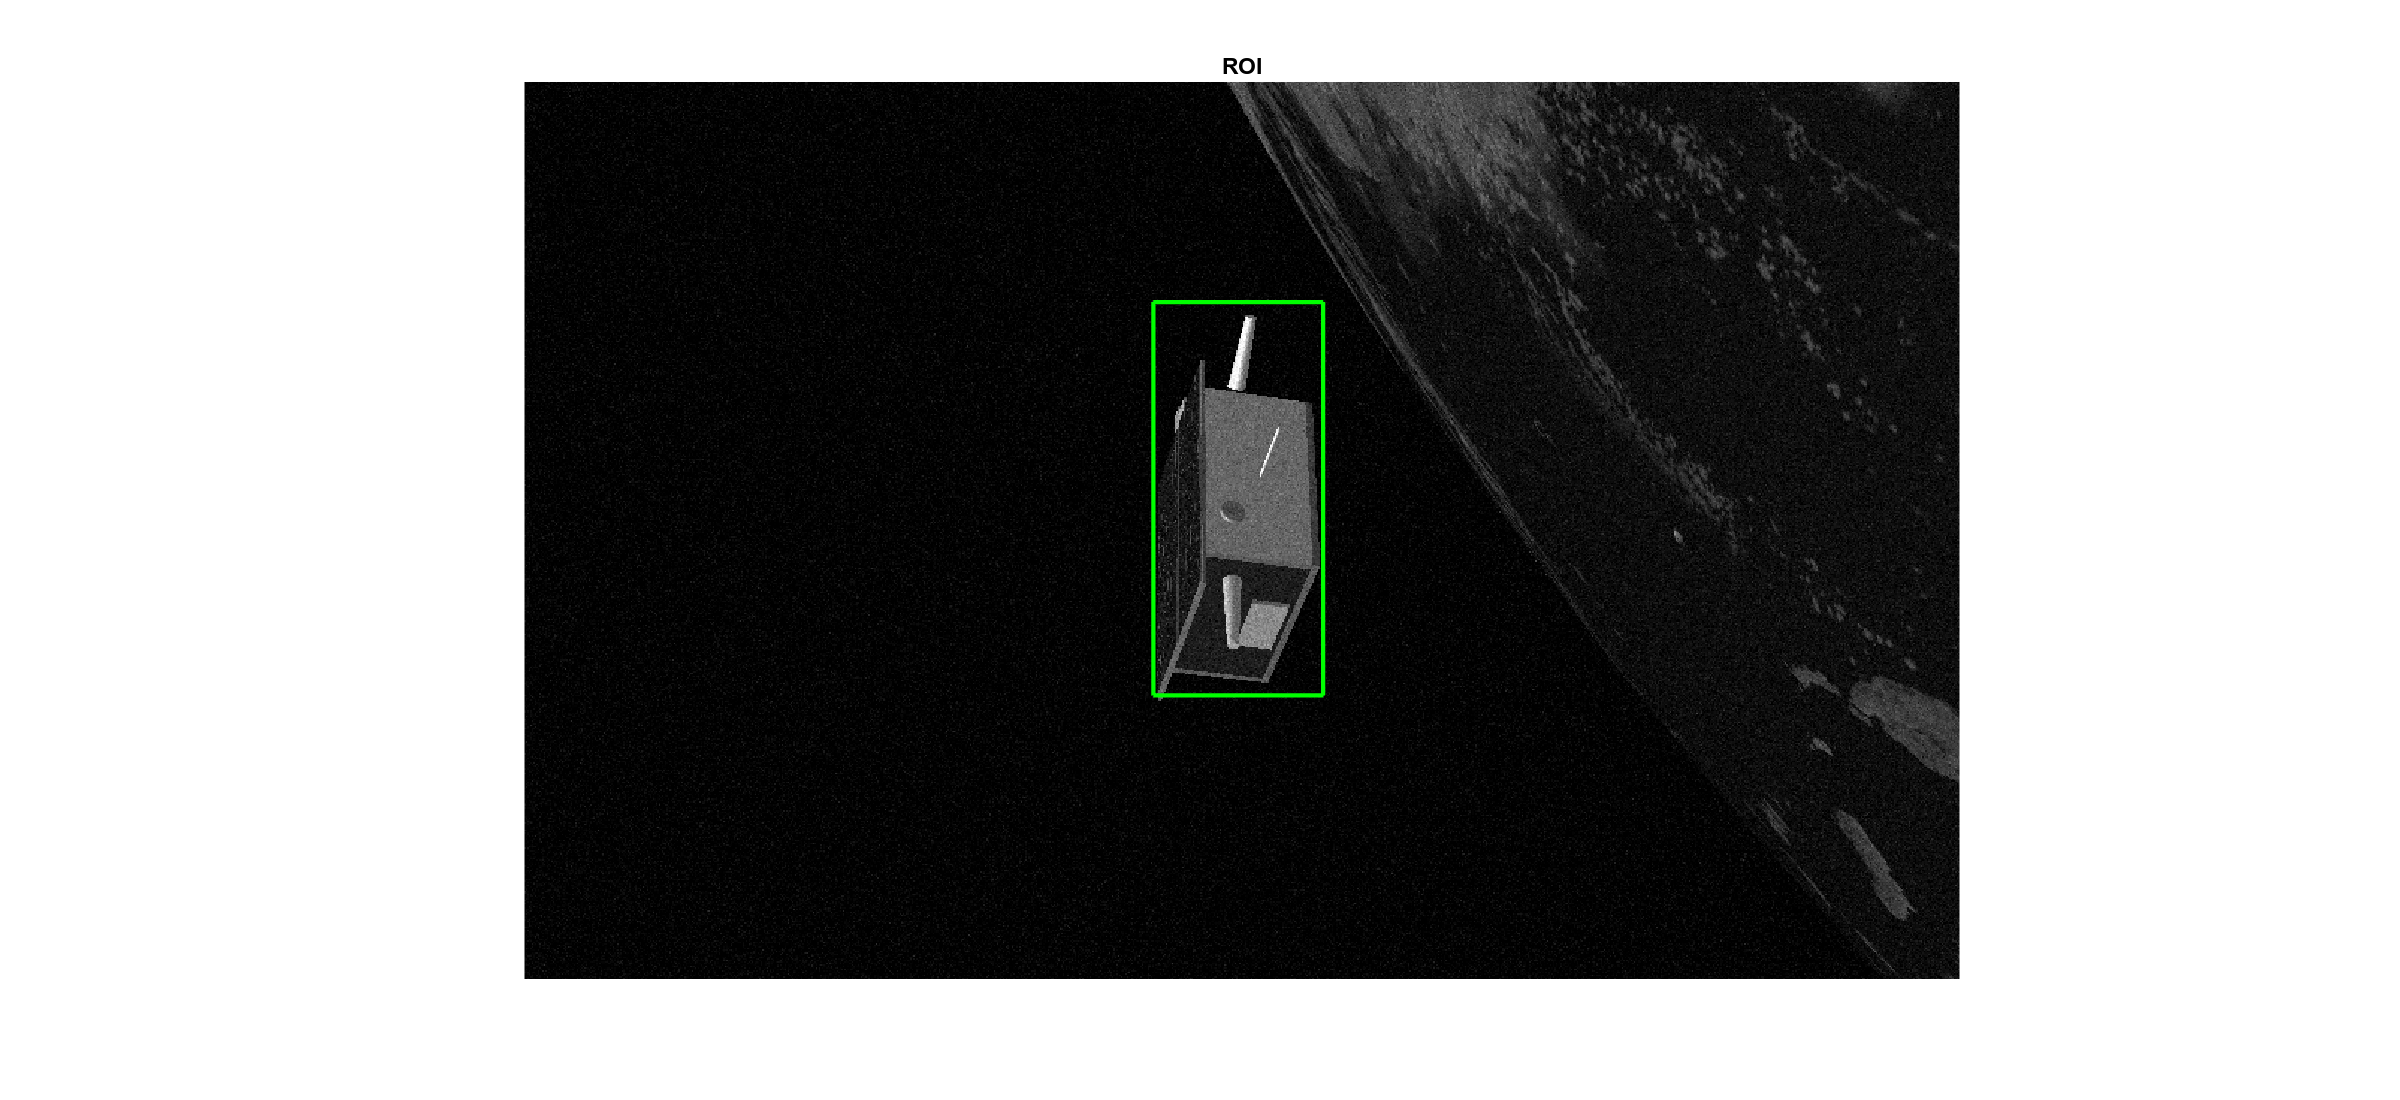
\includegraphics[width=0.45\textwidth]{gfx/results/prisma/113/9.png}}
  \qquad
  \subfloat[]{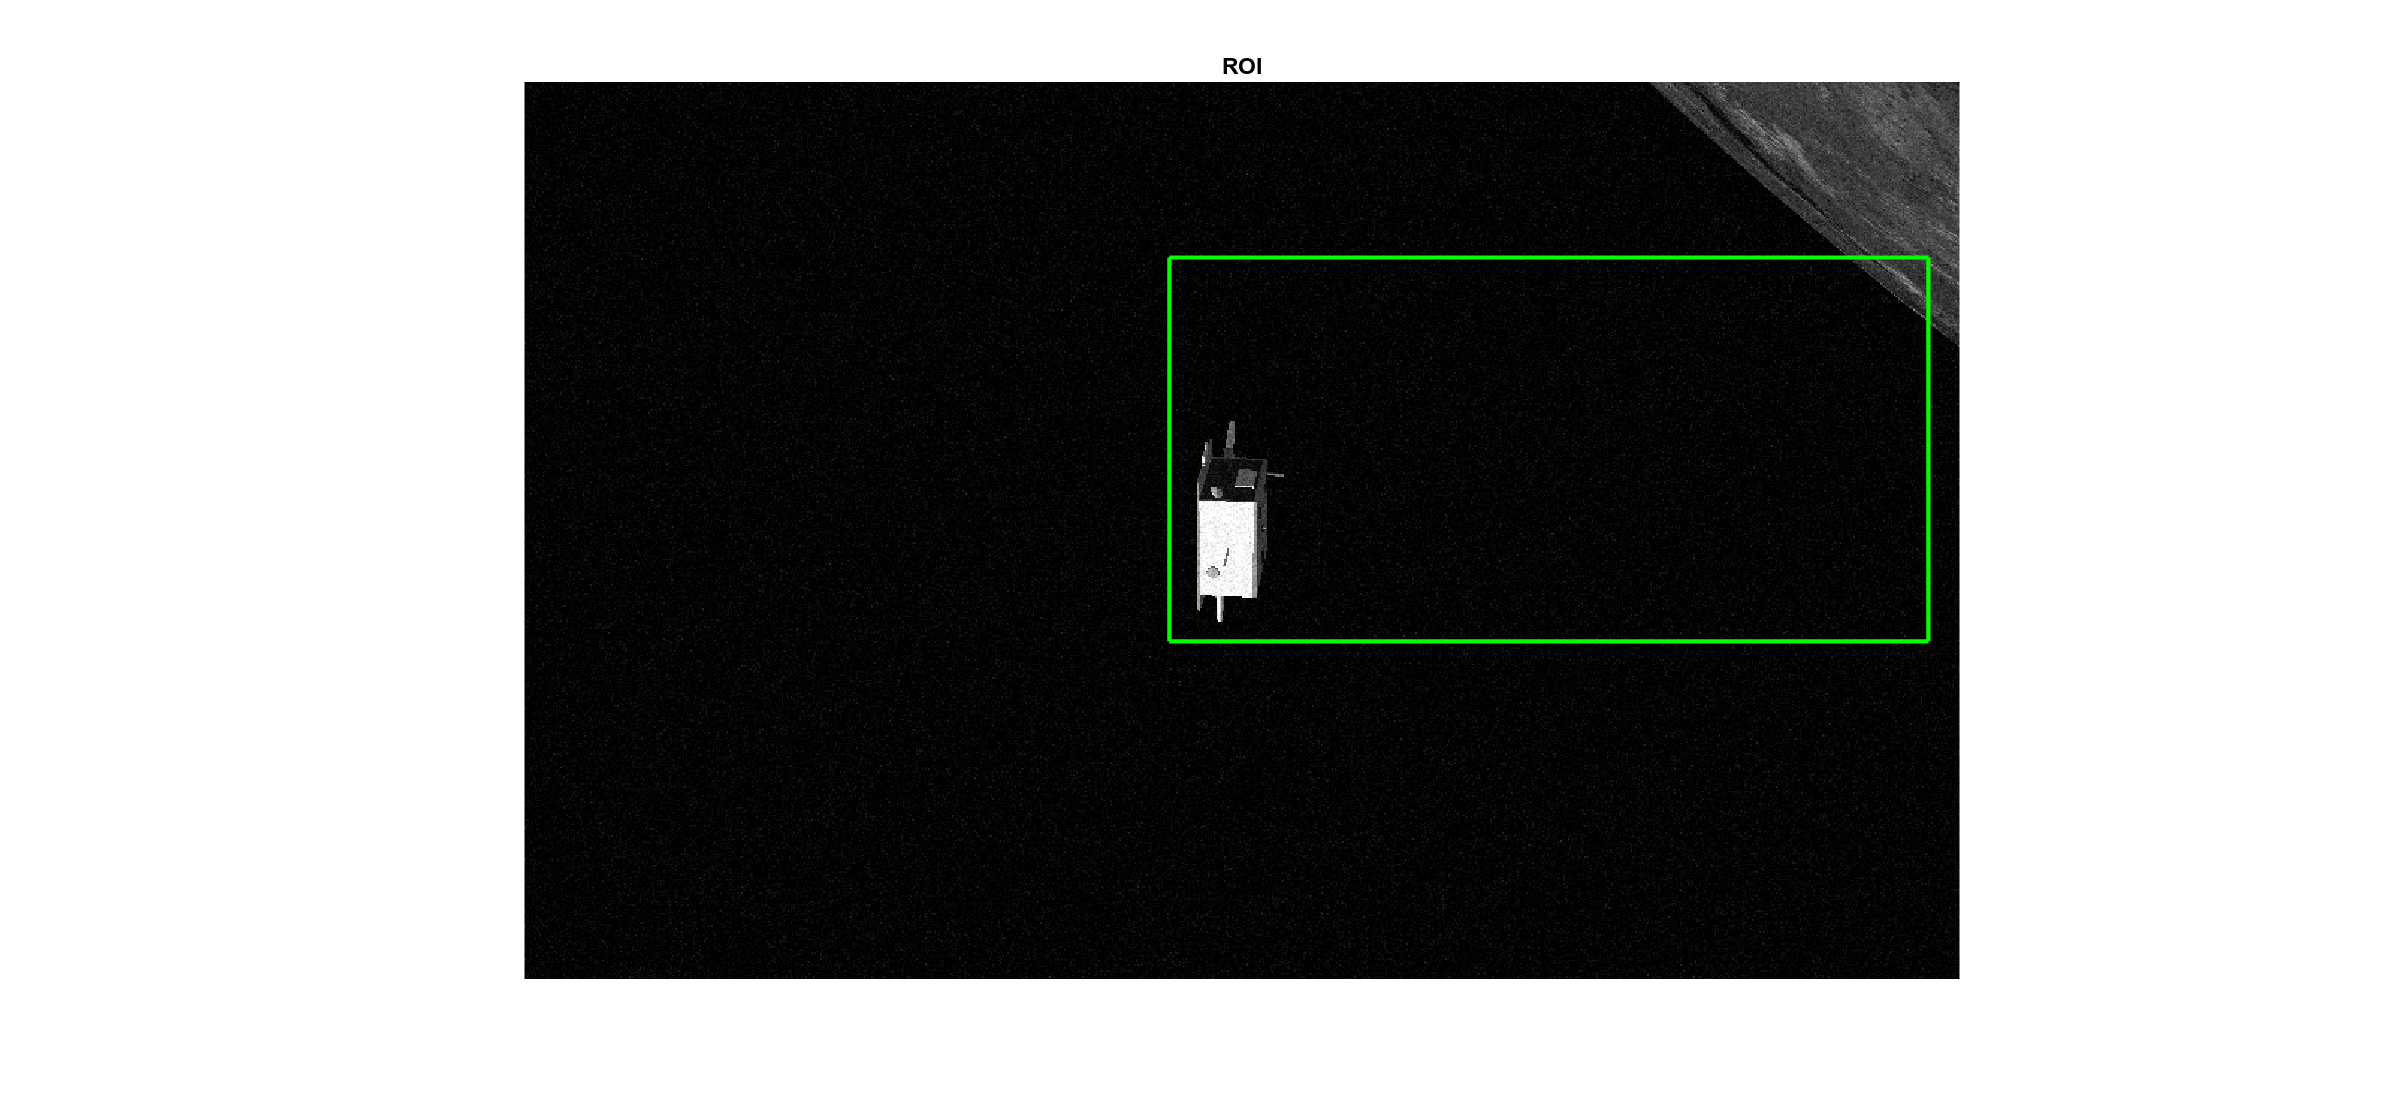
\includegraphics[width=0.45\textwidth]{gfx/results/prisma/114/9.png}}
  \qquad
  \subfloat[]{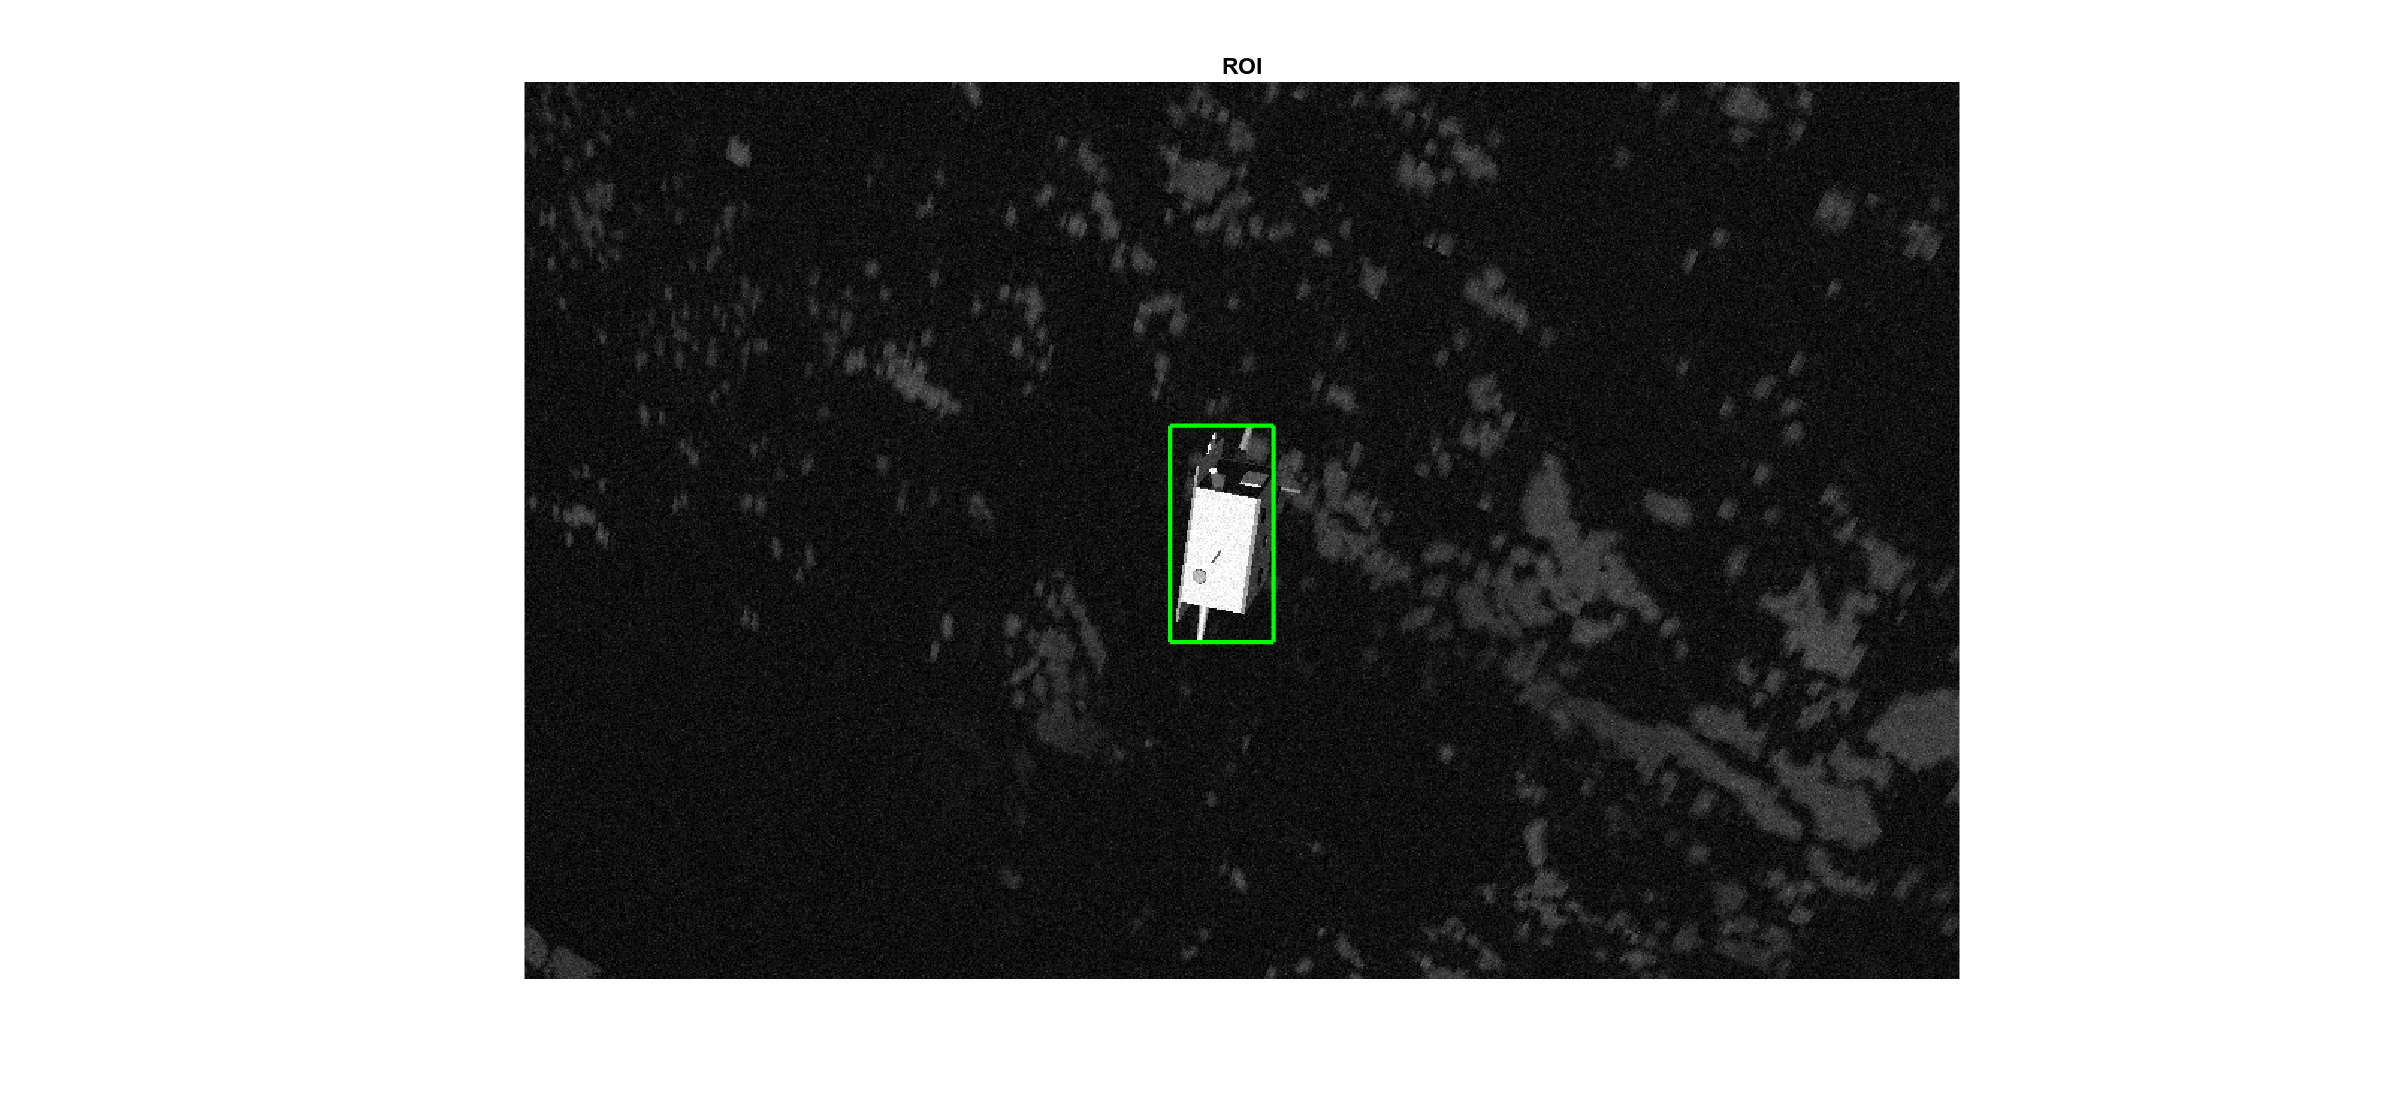
\includegraphics[width=0.45\textwidth]{gfx/results/prisma/115/9.png}}
  \qquad
  \subfloat[]{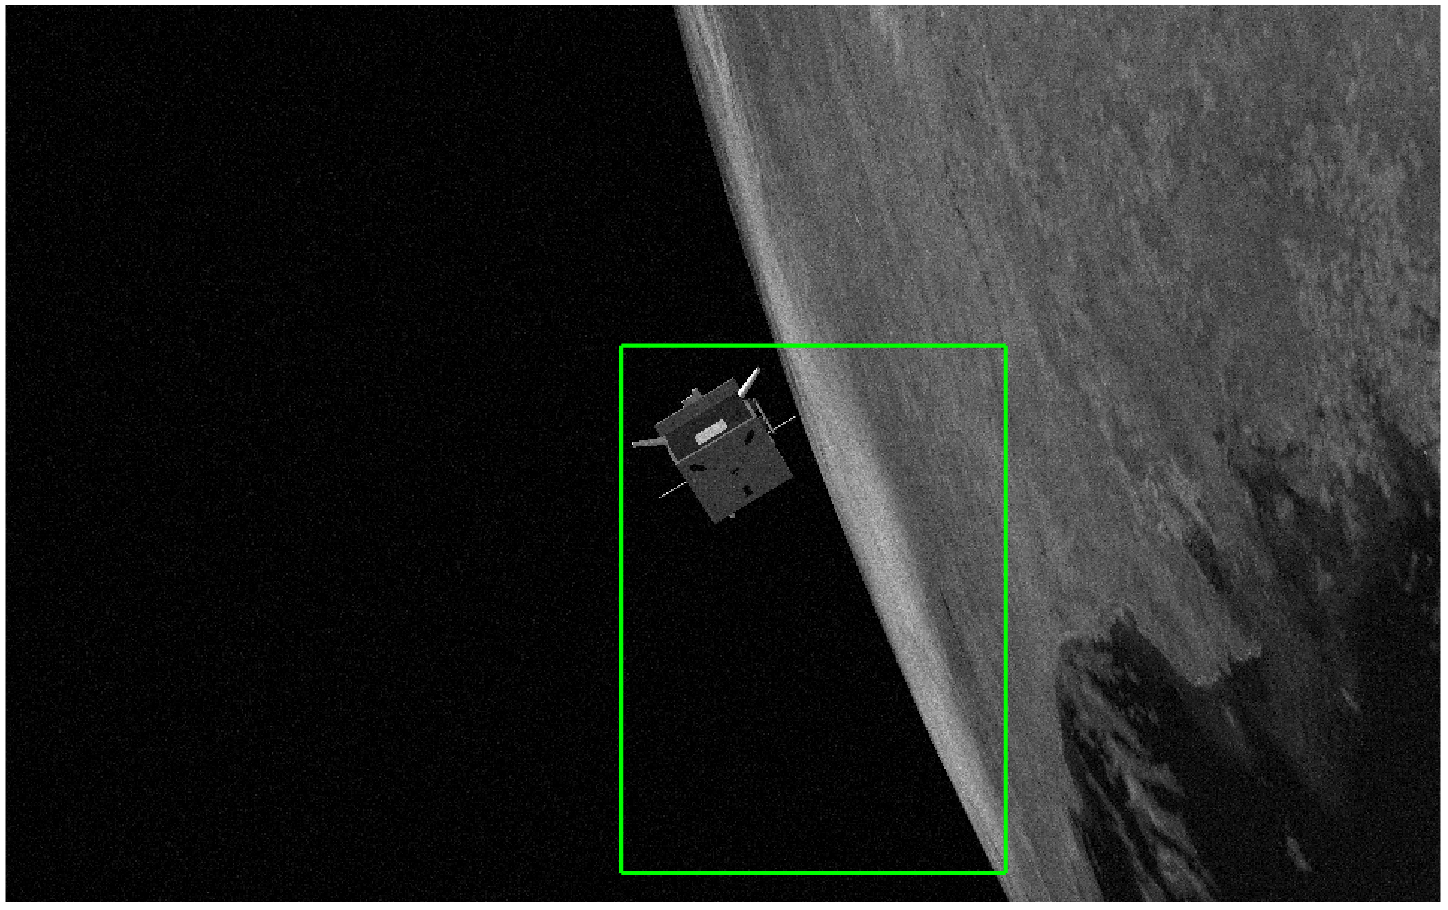
\includegraphics[width=0.45\textwidth]{gfx/results/prisma/116/9.png}}
  \qquad
  \subfloat[]{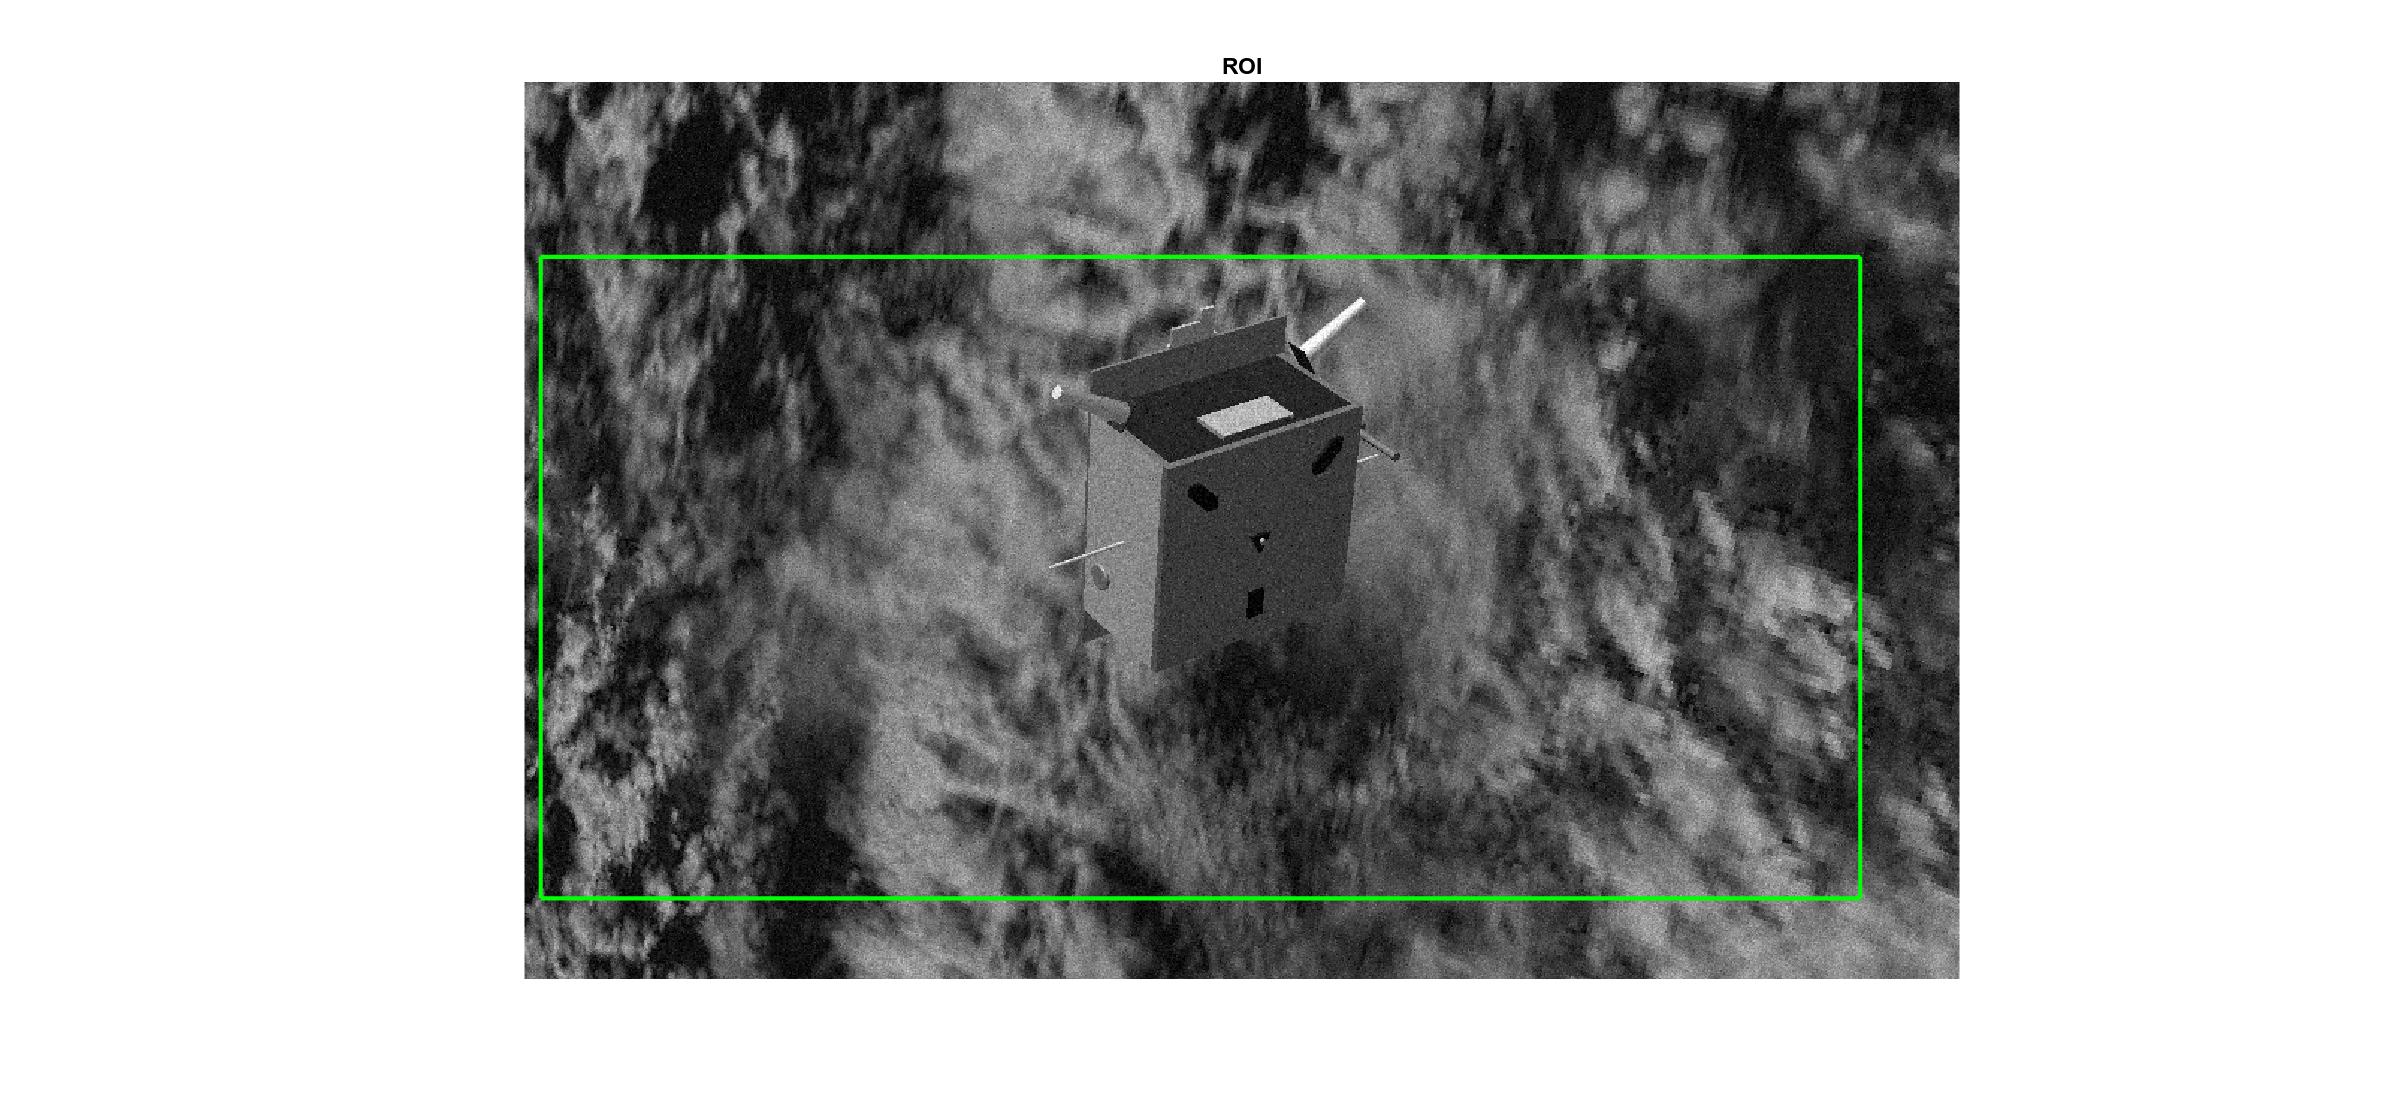
\includegraphics[width=0.45\textwidth]{gfx/results/prisma/117/9.png}}
  \qquad
  \caption{ROI detection tests}
  \label{fig:roiResults1}
\end{figure}

\begin{figure}[htbp]
  \centering
  \subfloat[]{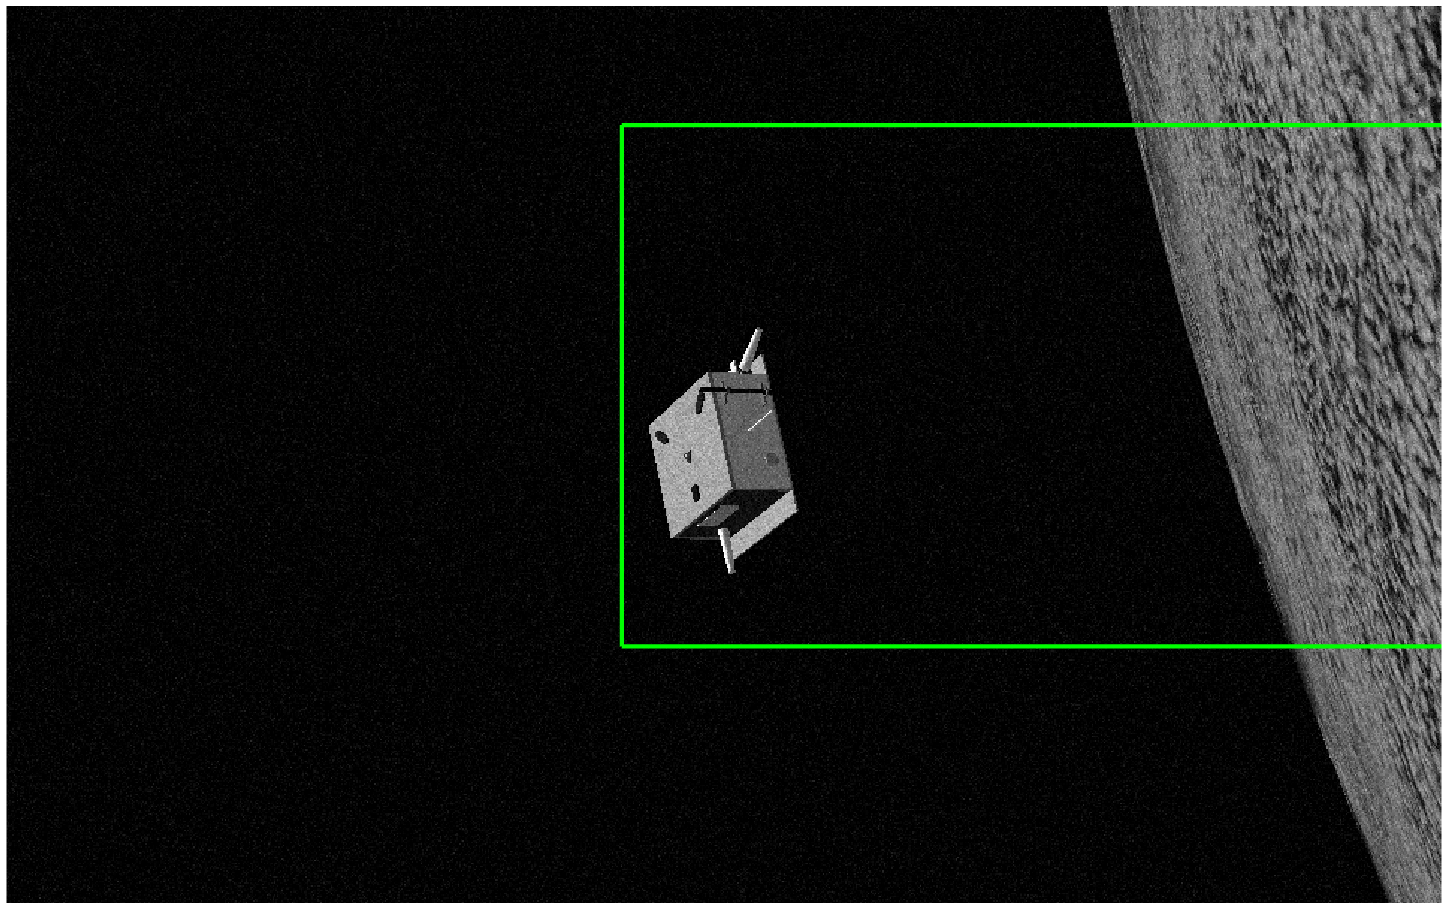
\includegraphics[width=0.45\textwidth]{gfx/results/prisma/101/9.png}}
  \qquad
  \subfloat[]{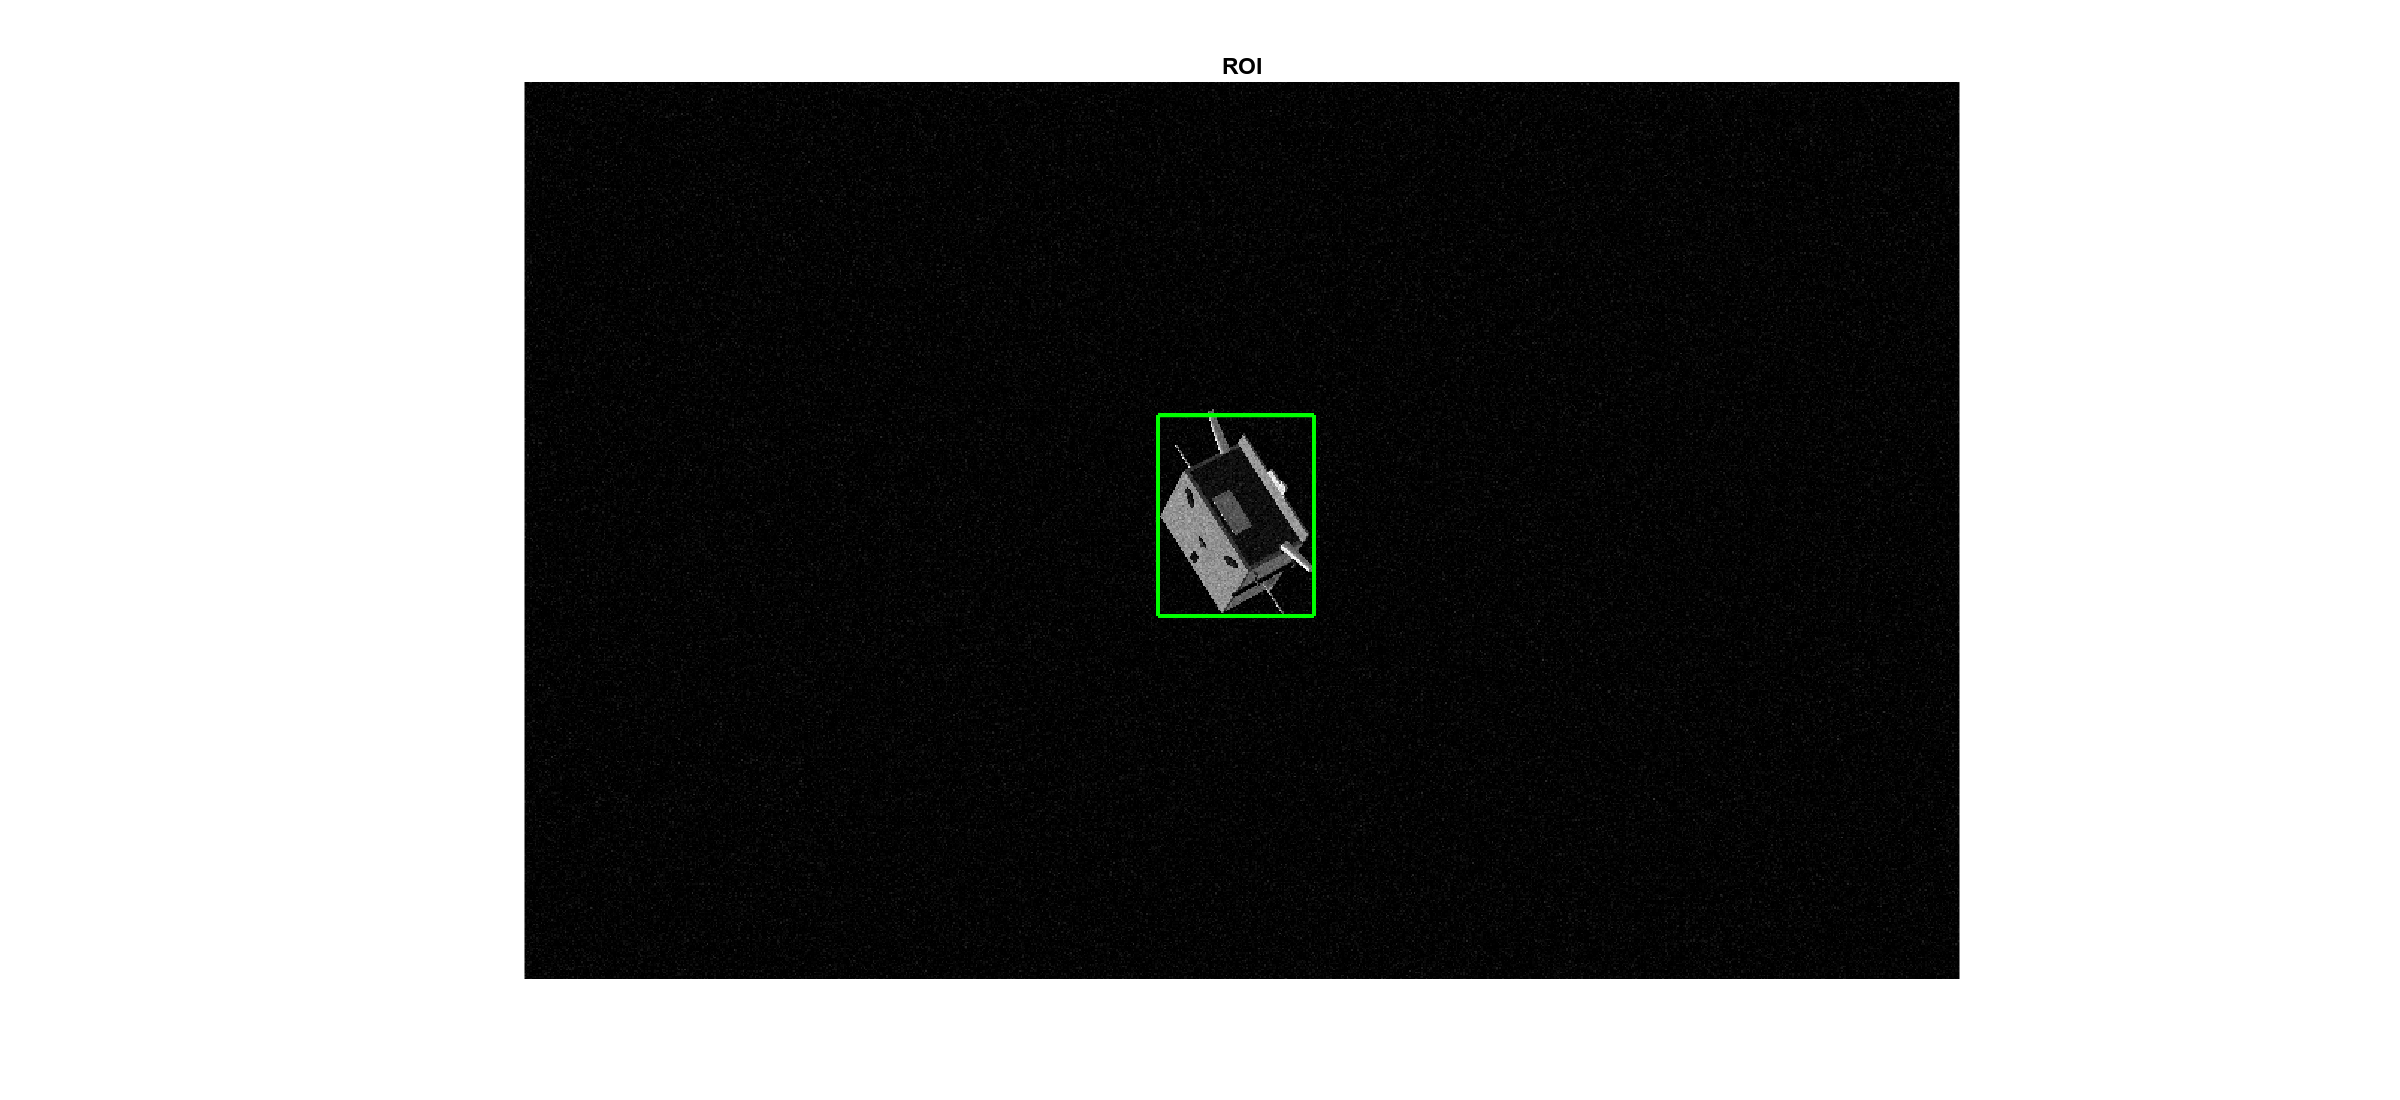
\includegraphics[width=0.45\textwidth]{gfx/results/prisma/161/9.png}}
  \qquad
  \subfloat[]{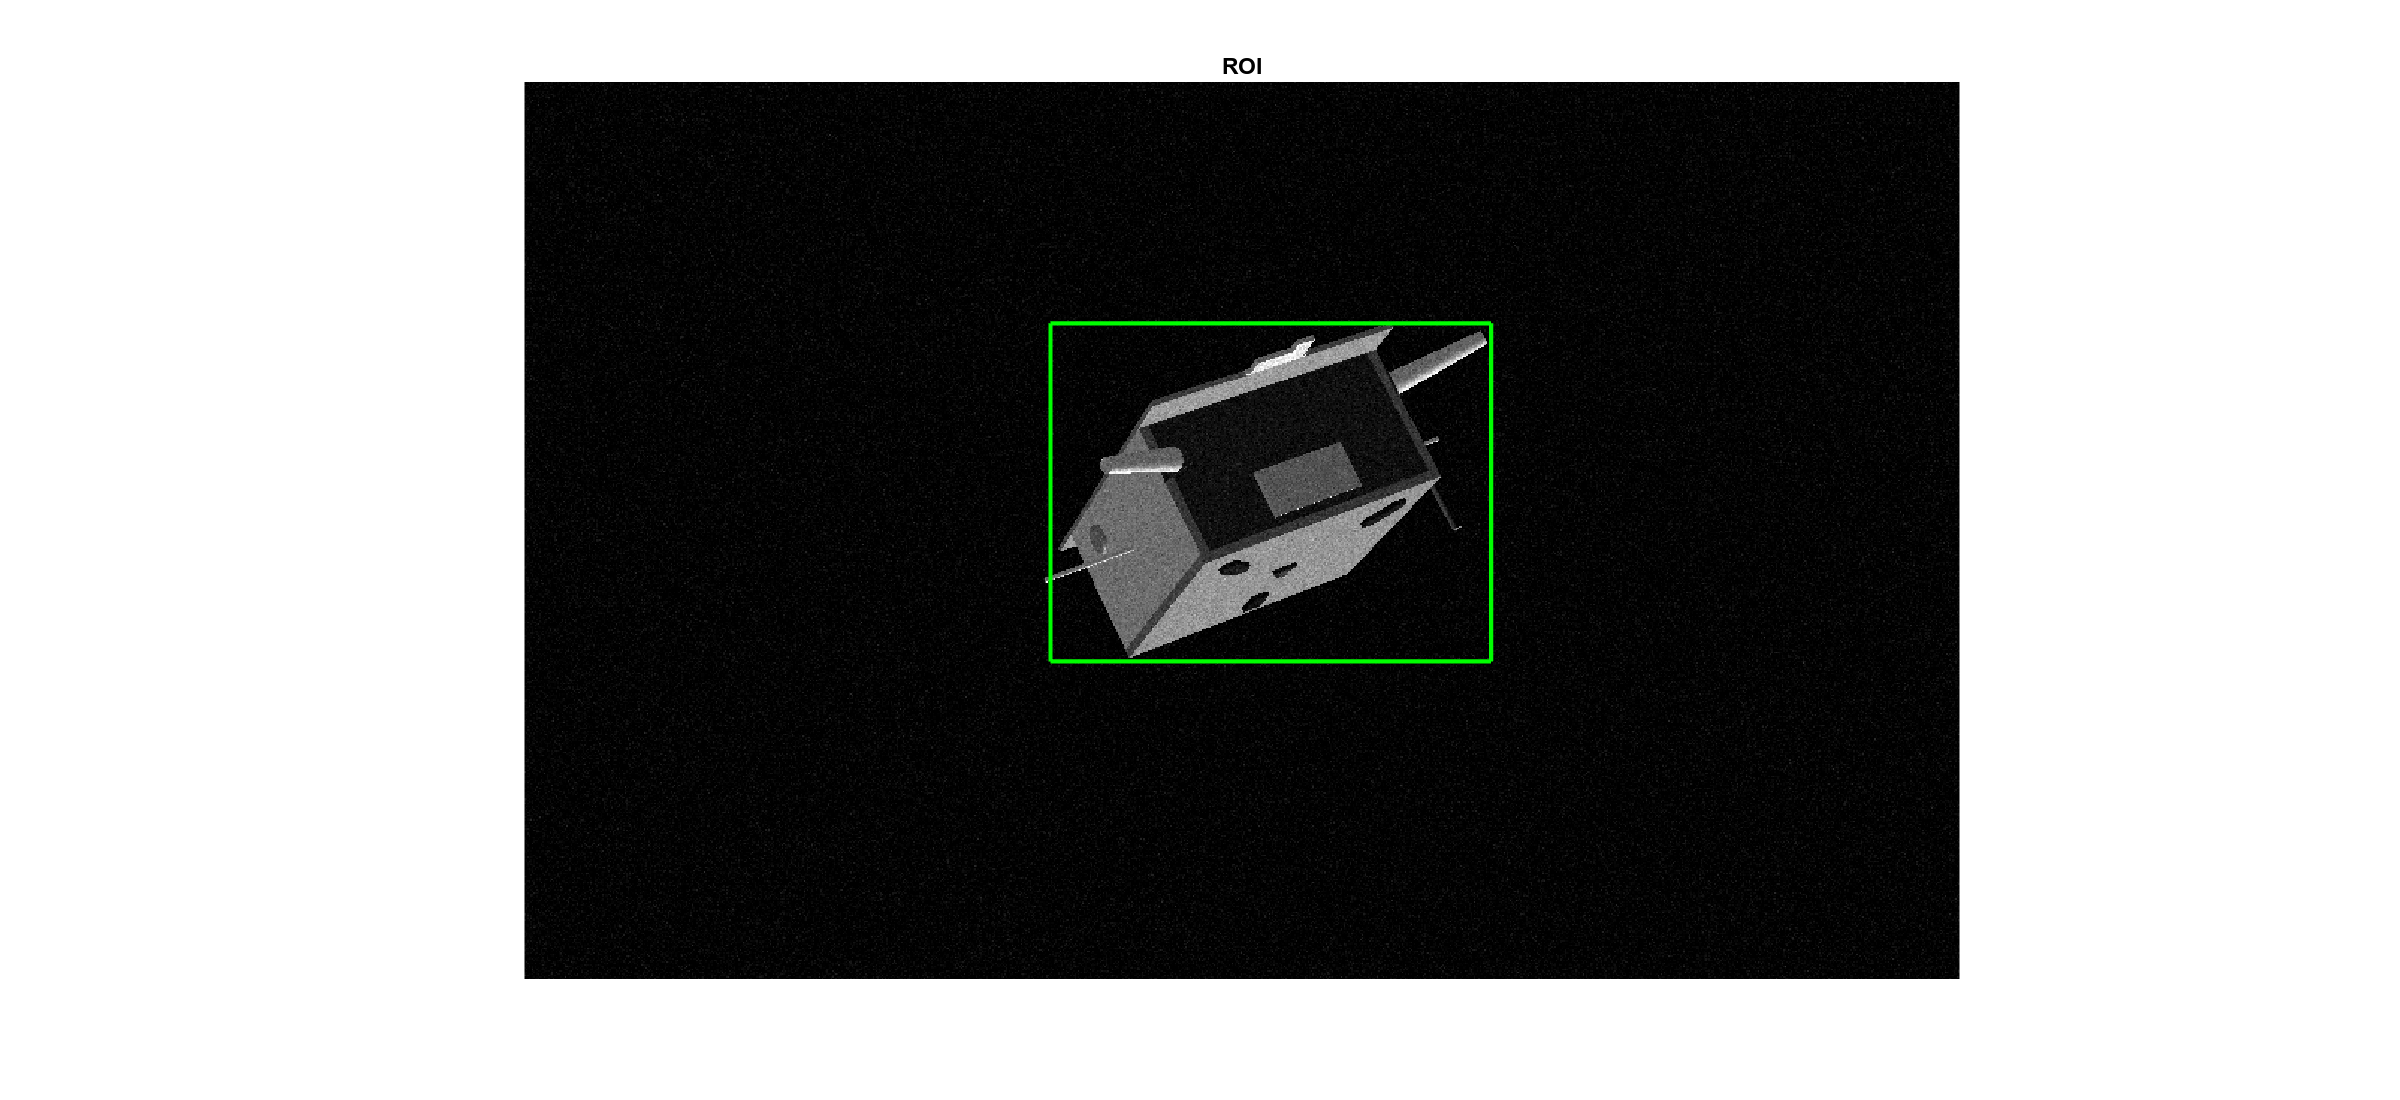
\includegraphics[width=0.45\textwidth]{gfx/results/prisma/162/9.png}}
  \qquad
  \subfloat[]{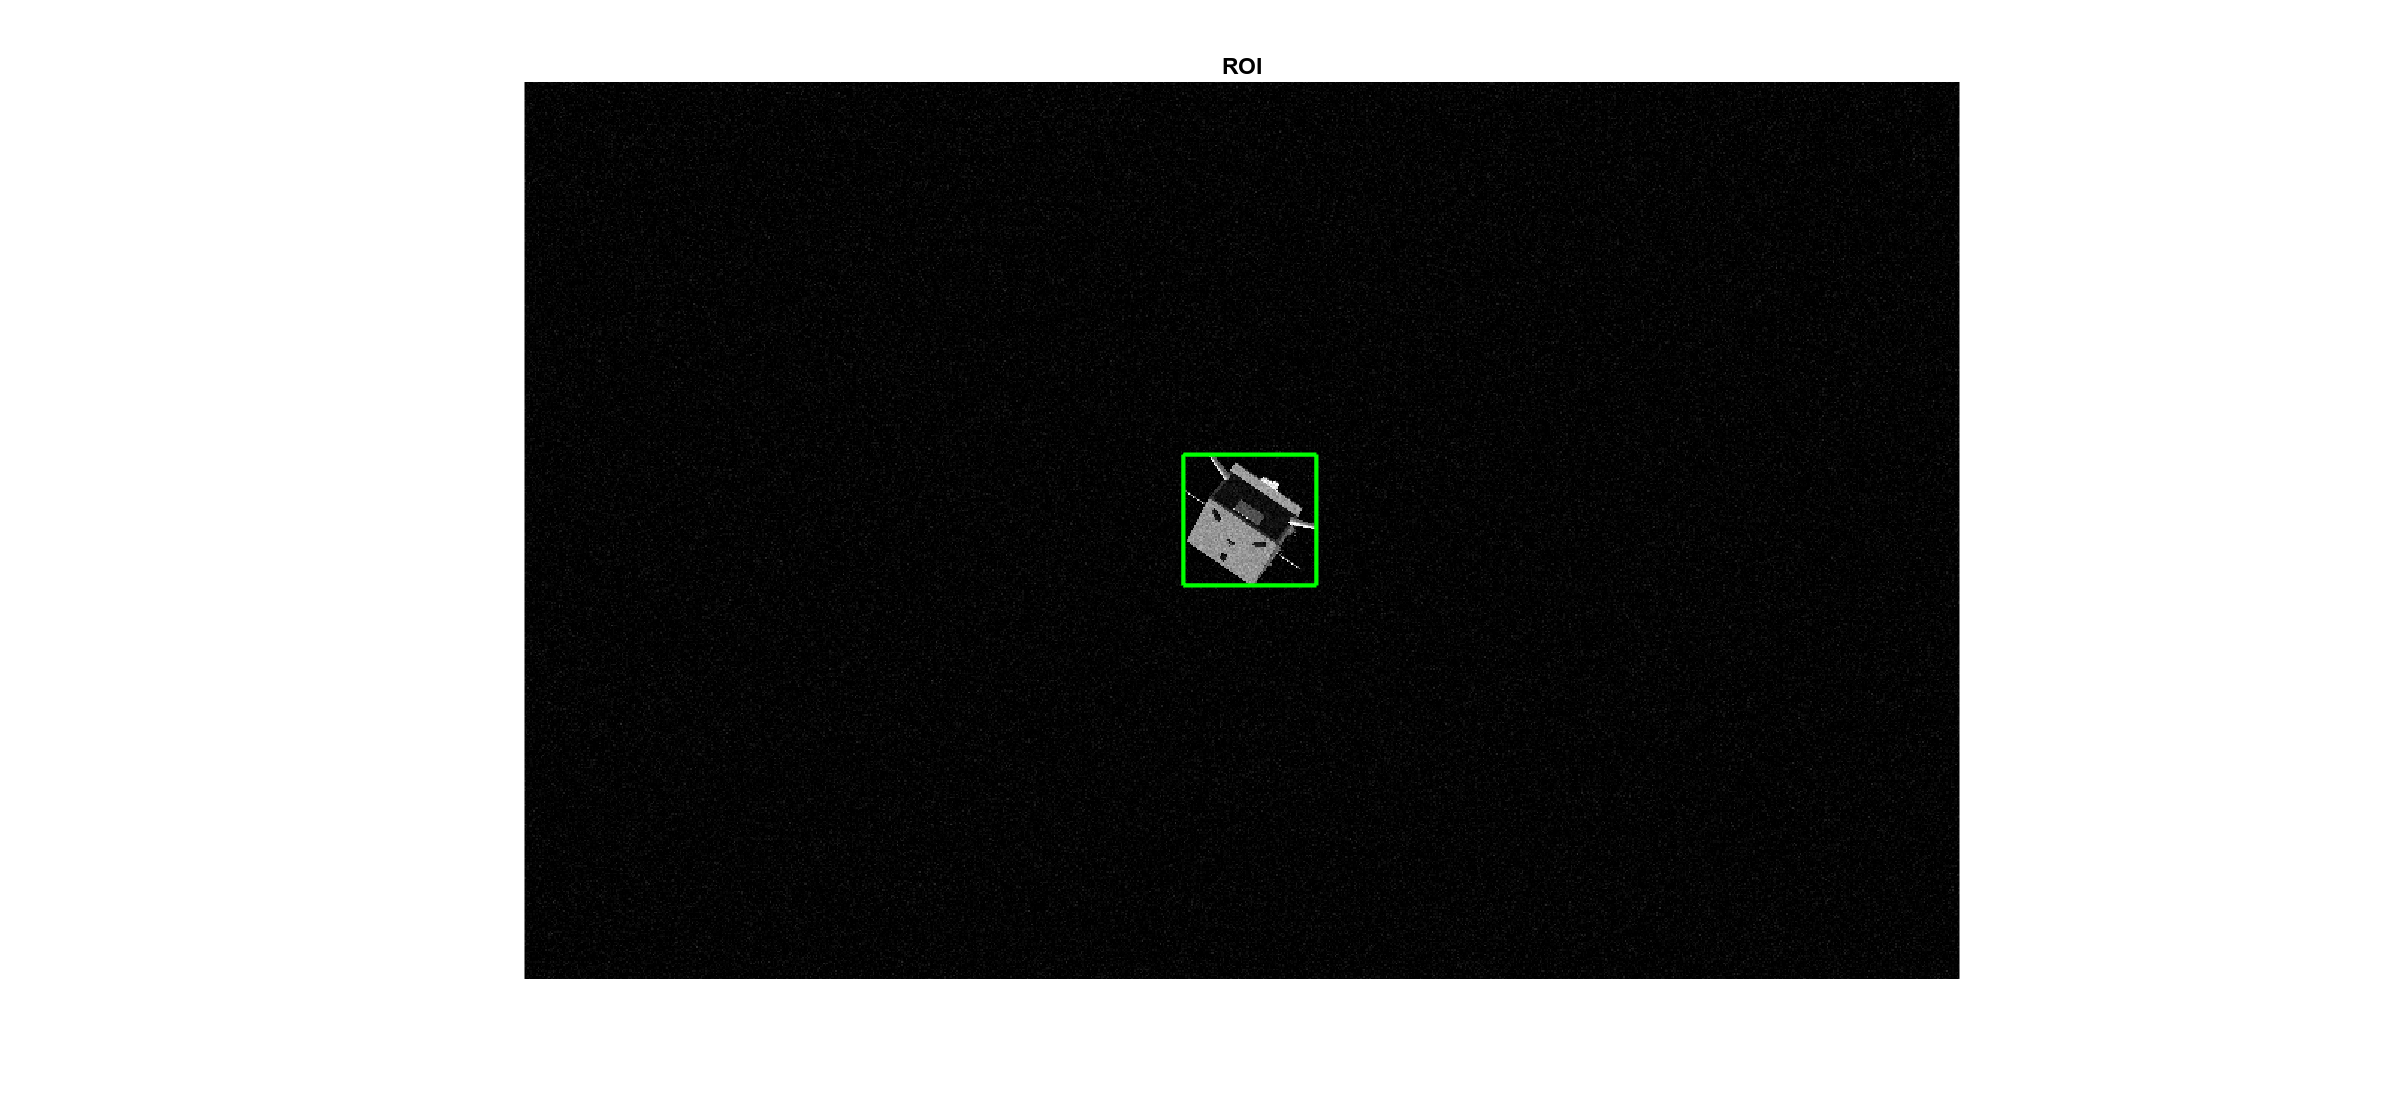
\includegraphics[width=0.45\textwidth]{gfx/results/prisma/163/9.png}}
  \qquad
  \subfloat[]{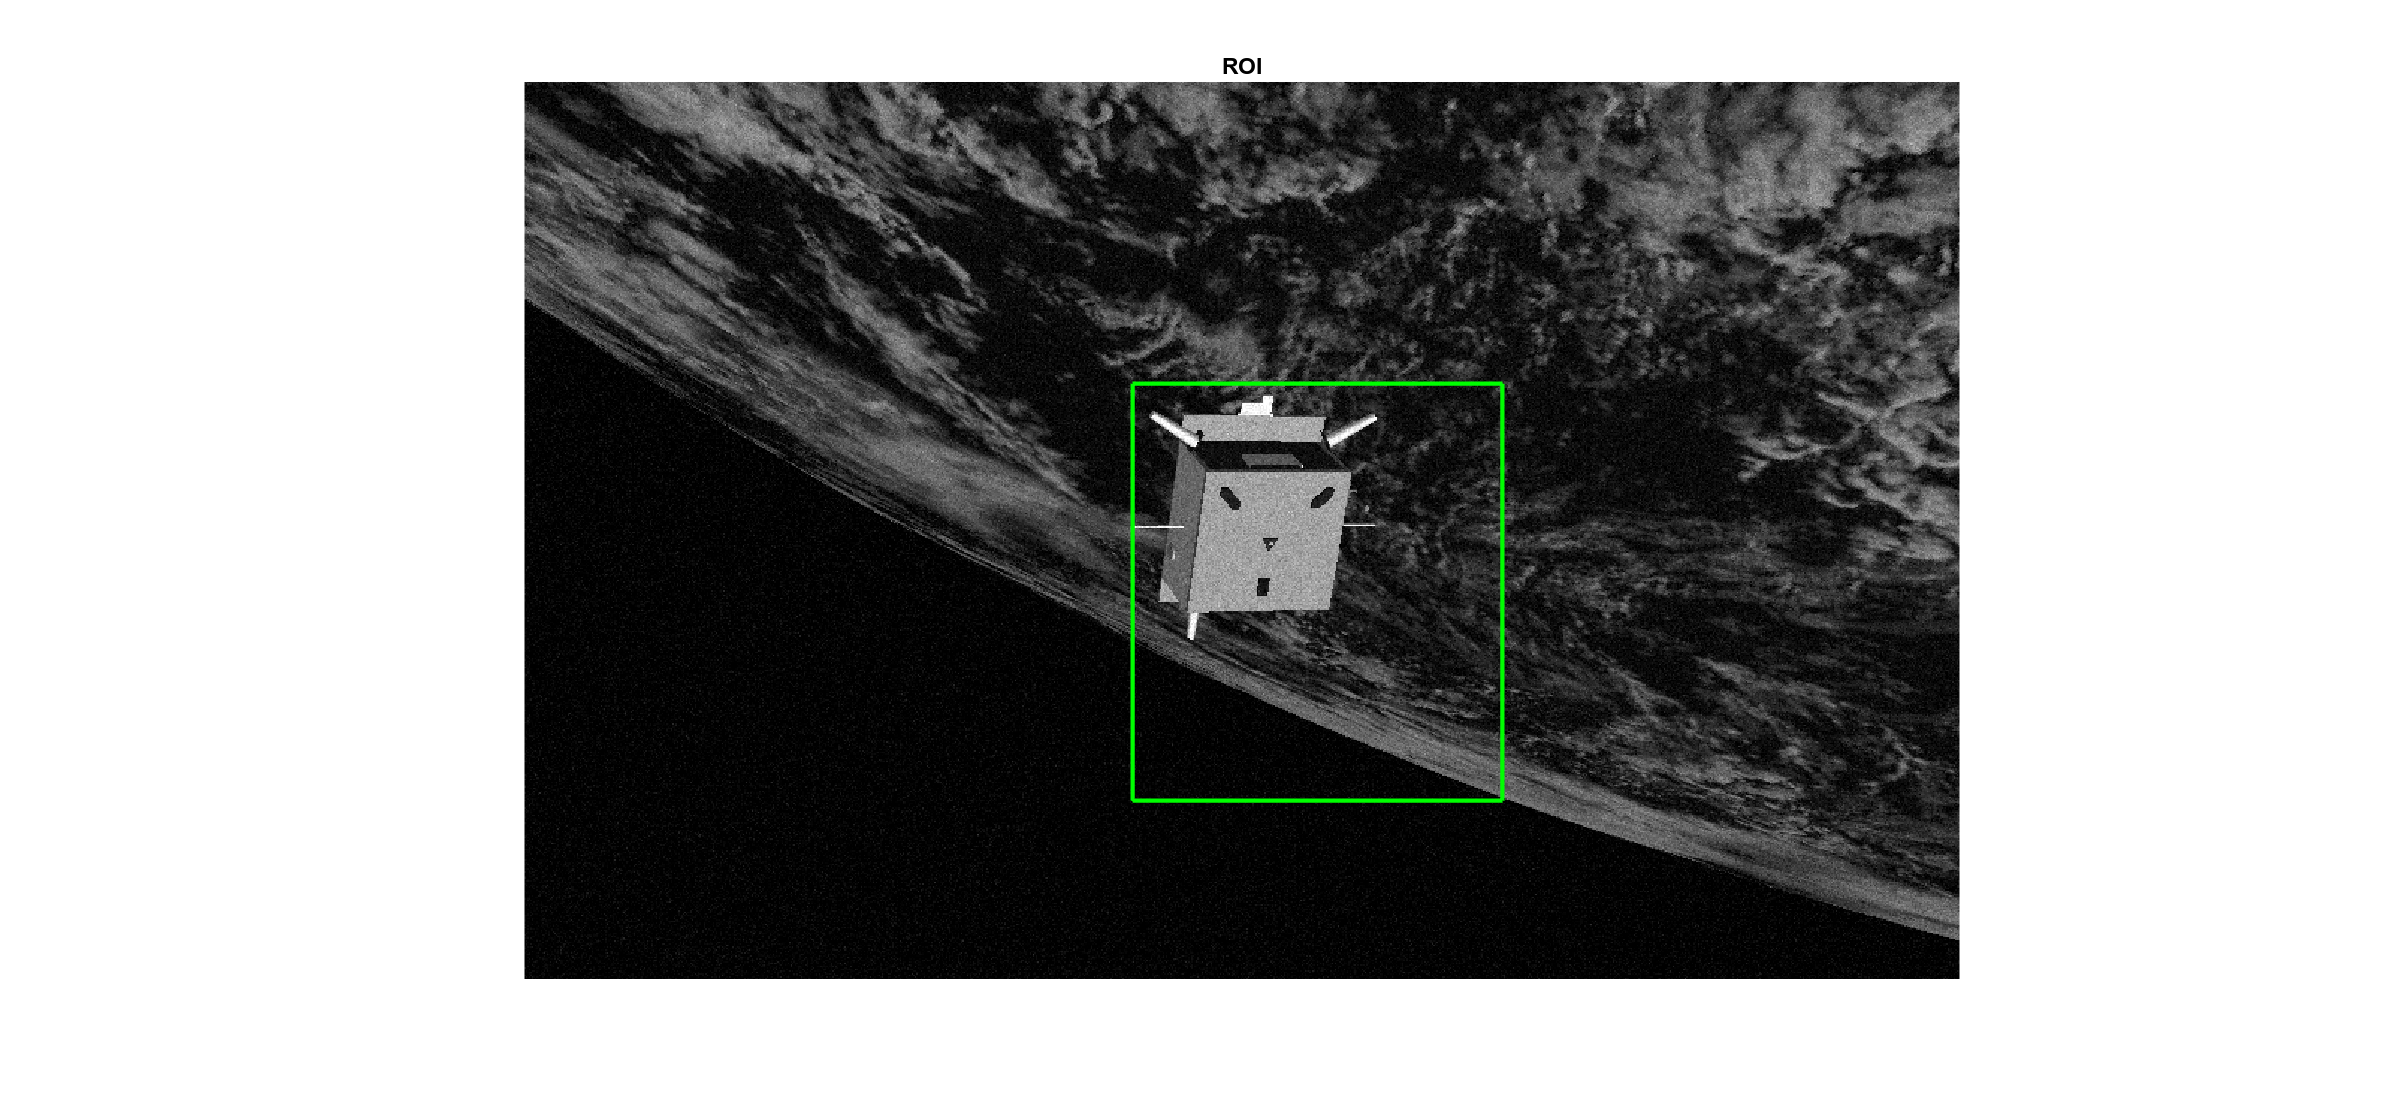
\includegraphics[width=0.45\textwidth]{gfx/results/prisma/164/9.png}}
  \qquad
  \subfloat[]{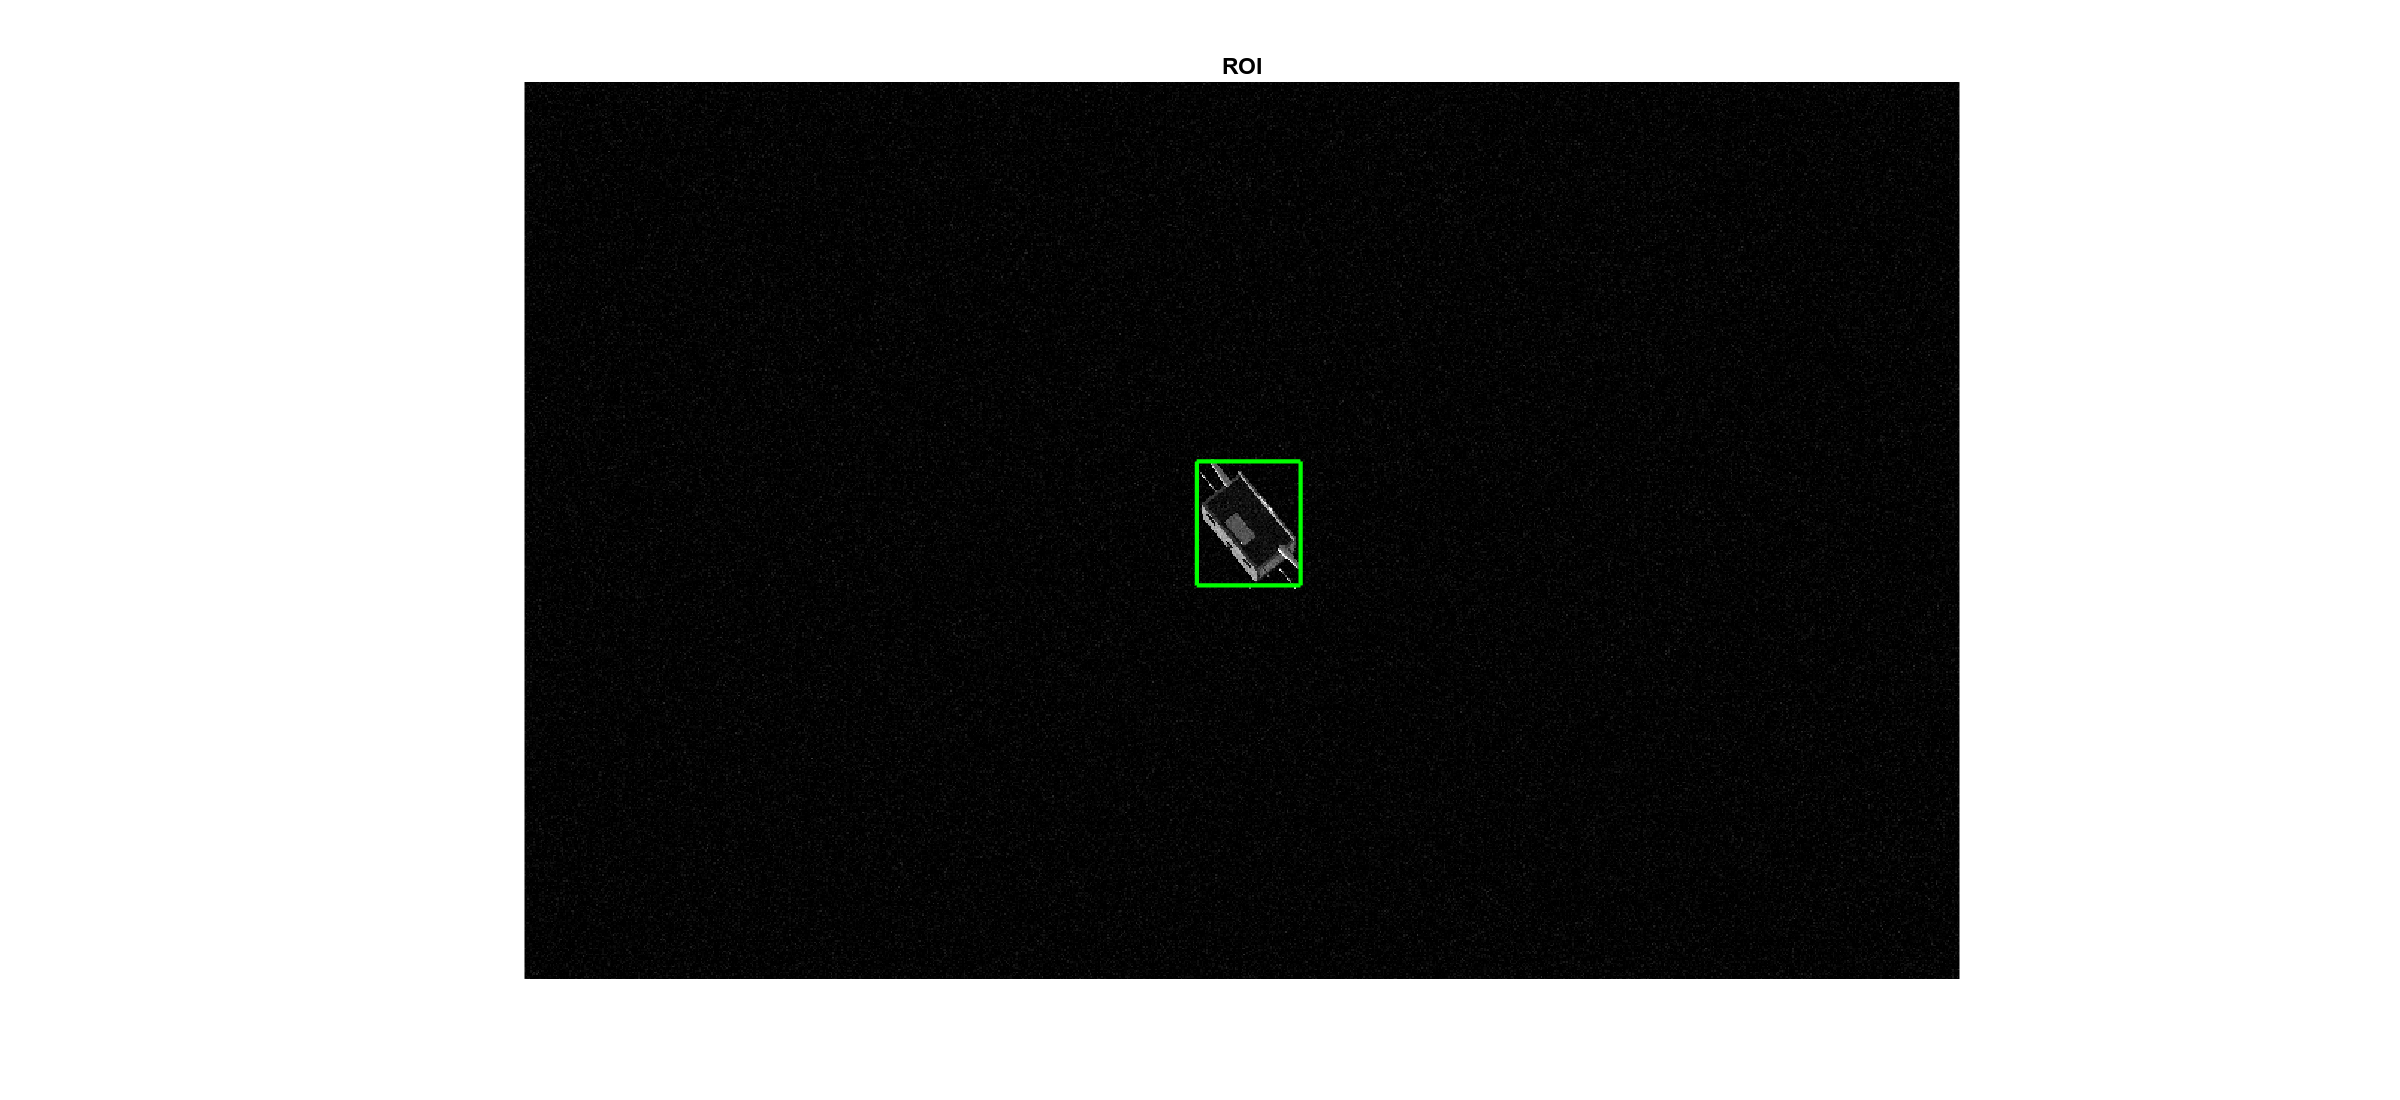
\includegraphics[width=0.45\textwidth]{gfx/results/prisma/165/9.png}}
  \qquad
  \subfloat[]{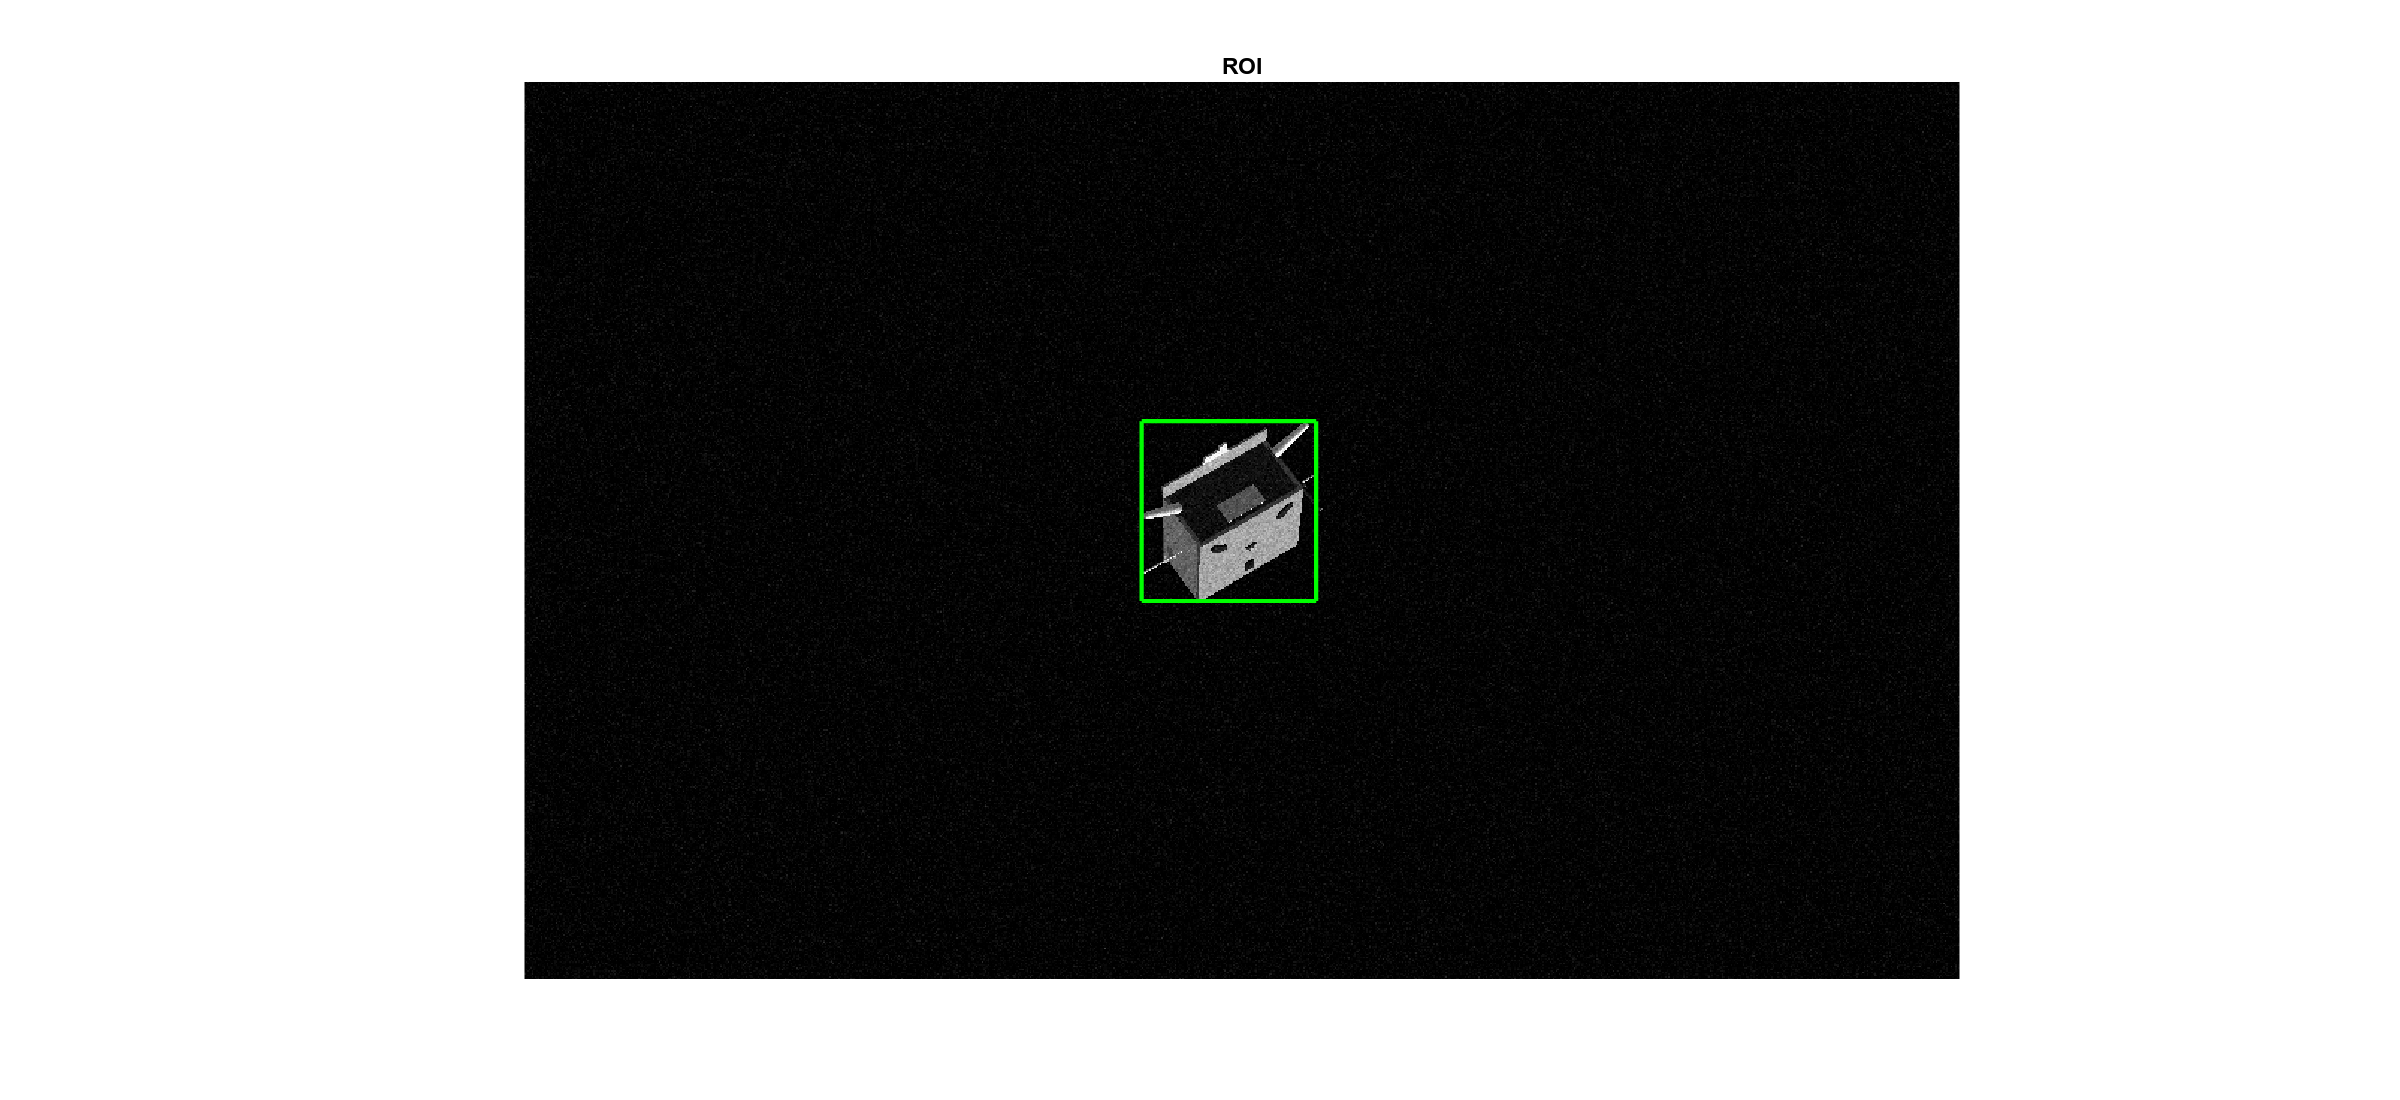
\includegraphics[width=0.45\textwidth]{gfx/results/prisma/166/9.png}}
  \qquad
  \subfloat[]{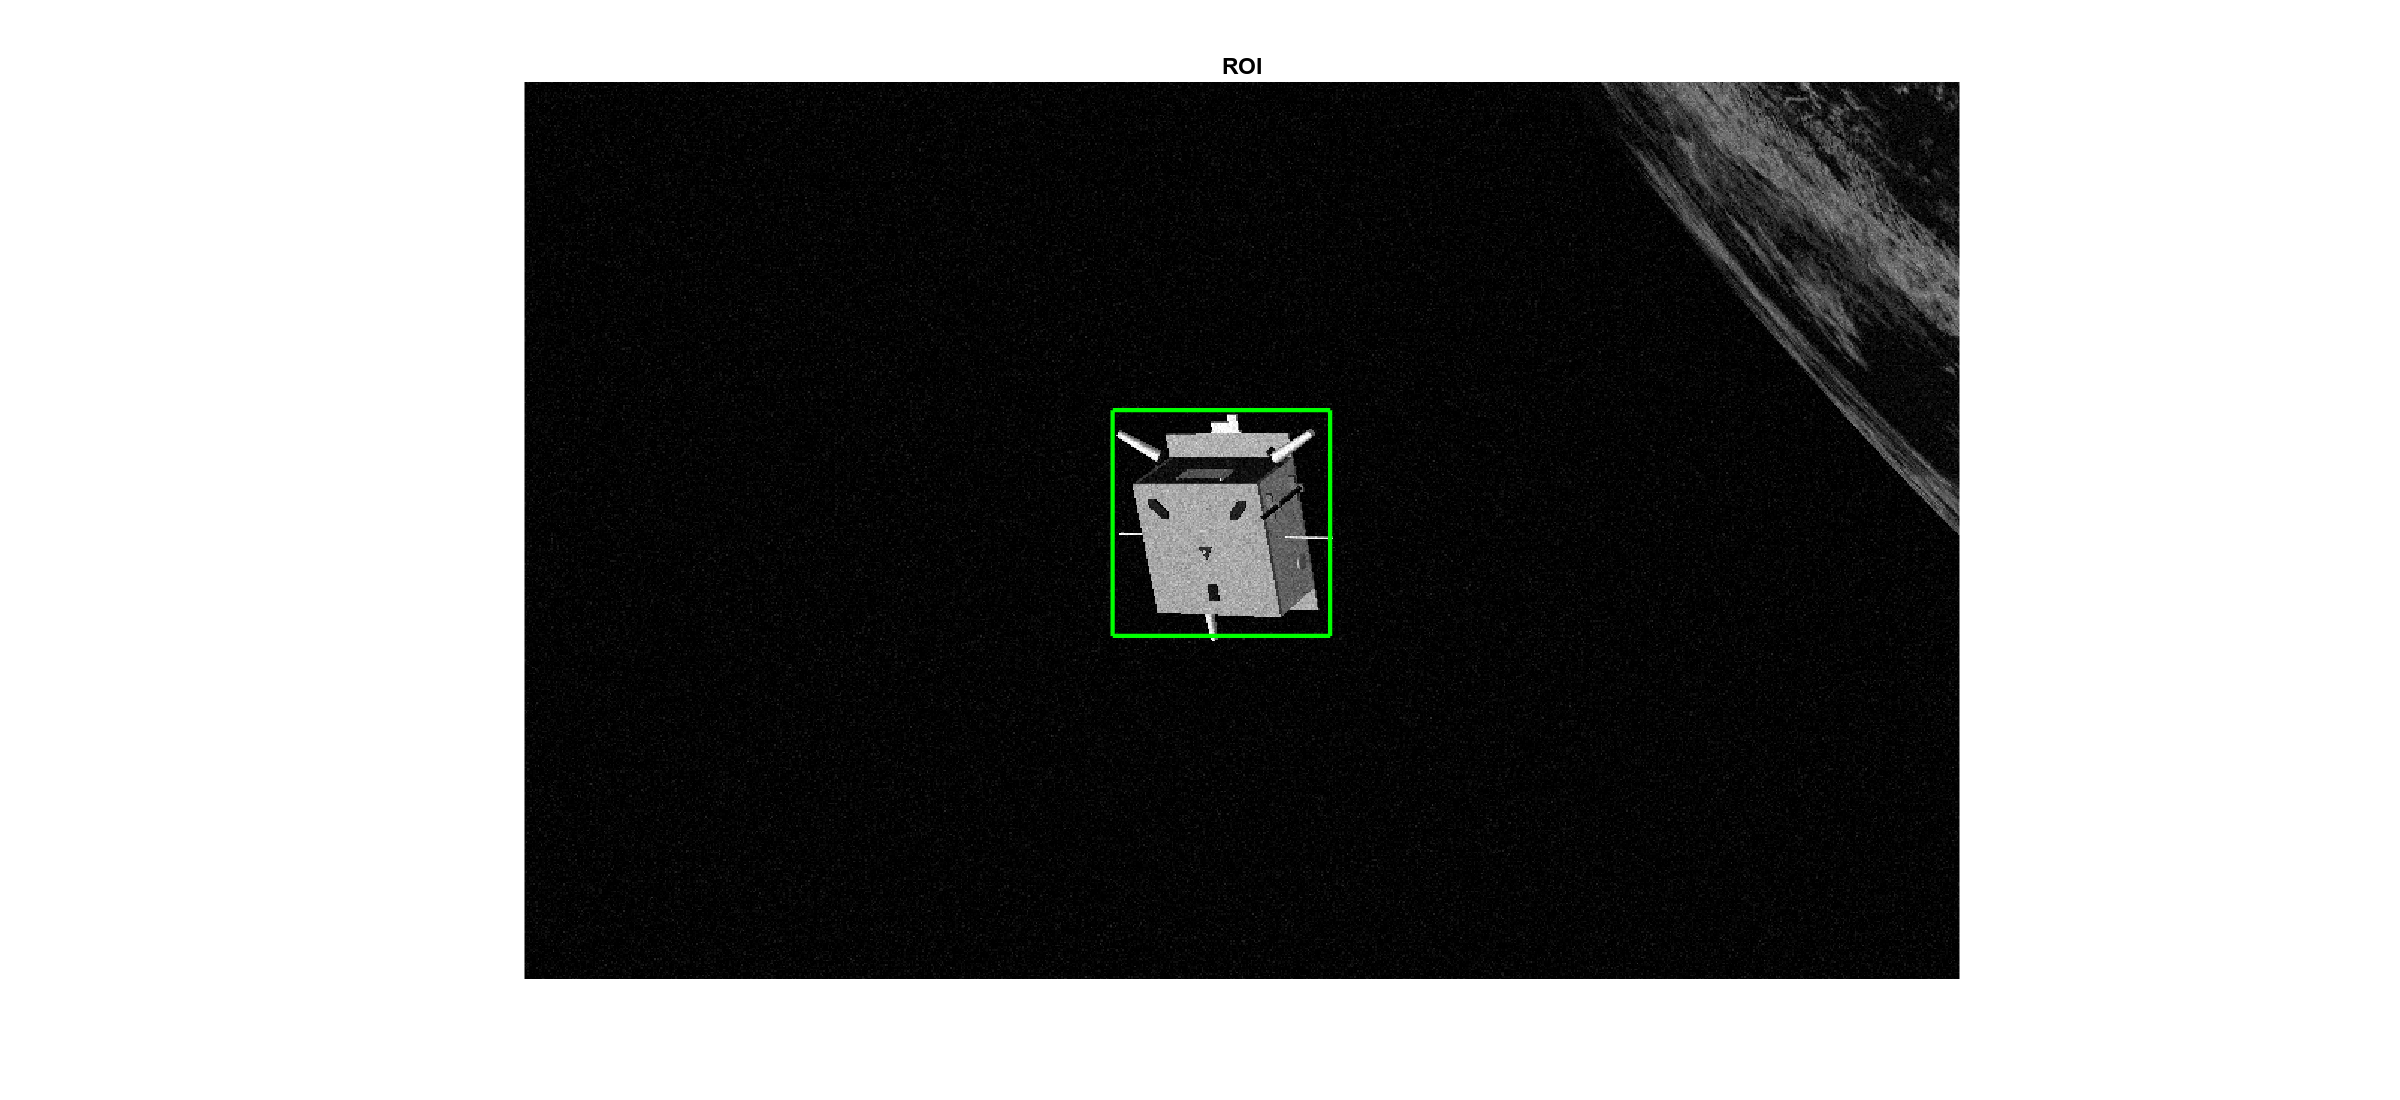
\includegraphics[width=0.45\textwidth]{gfx/results/prisma/169/9.png}}
  \qquad
  \caption{ROI detection tests}
  \label{fig:roiResults2}
\end{figure}

\begin{figure}[htbp]
  \centering
  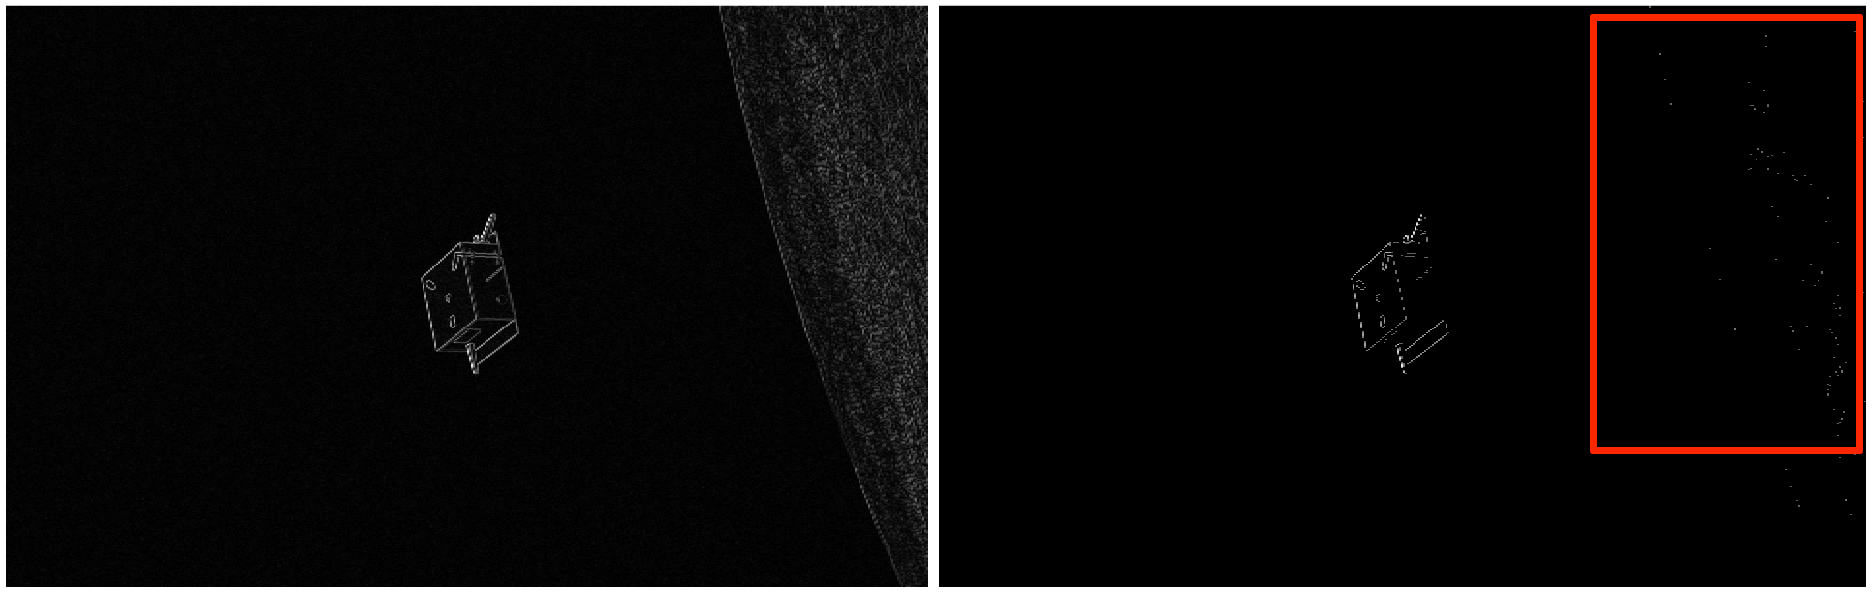
\includegraphics[width=1.0\textwidth]{gfx/results/prisma/101/8Select.png}
  \caption{Gradient image of figure \ref{fig:roiResults1}a}
\end{figure}

\begin{figure}[htbp]
  \centering
  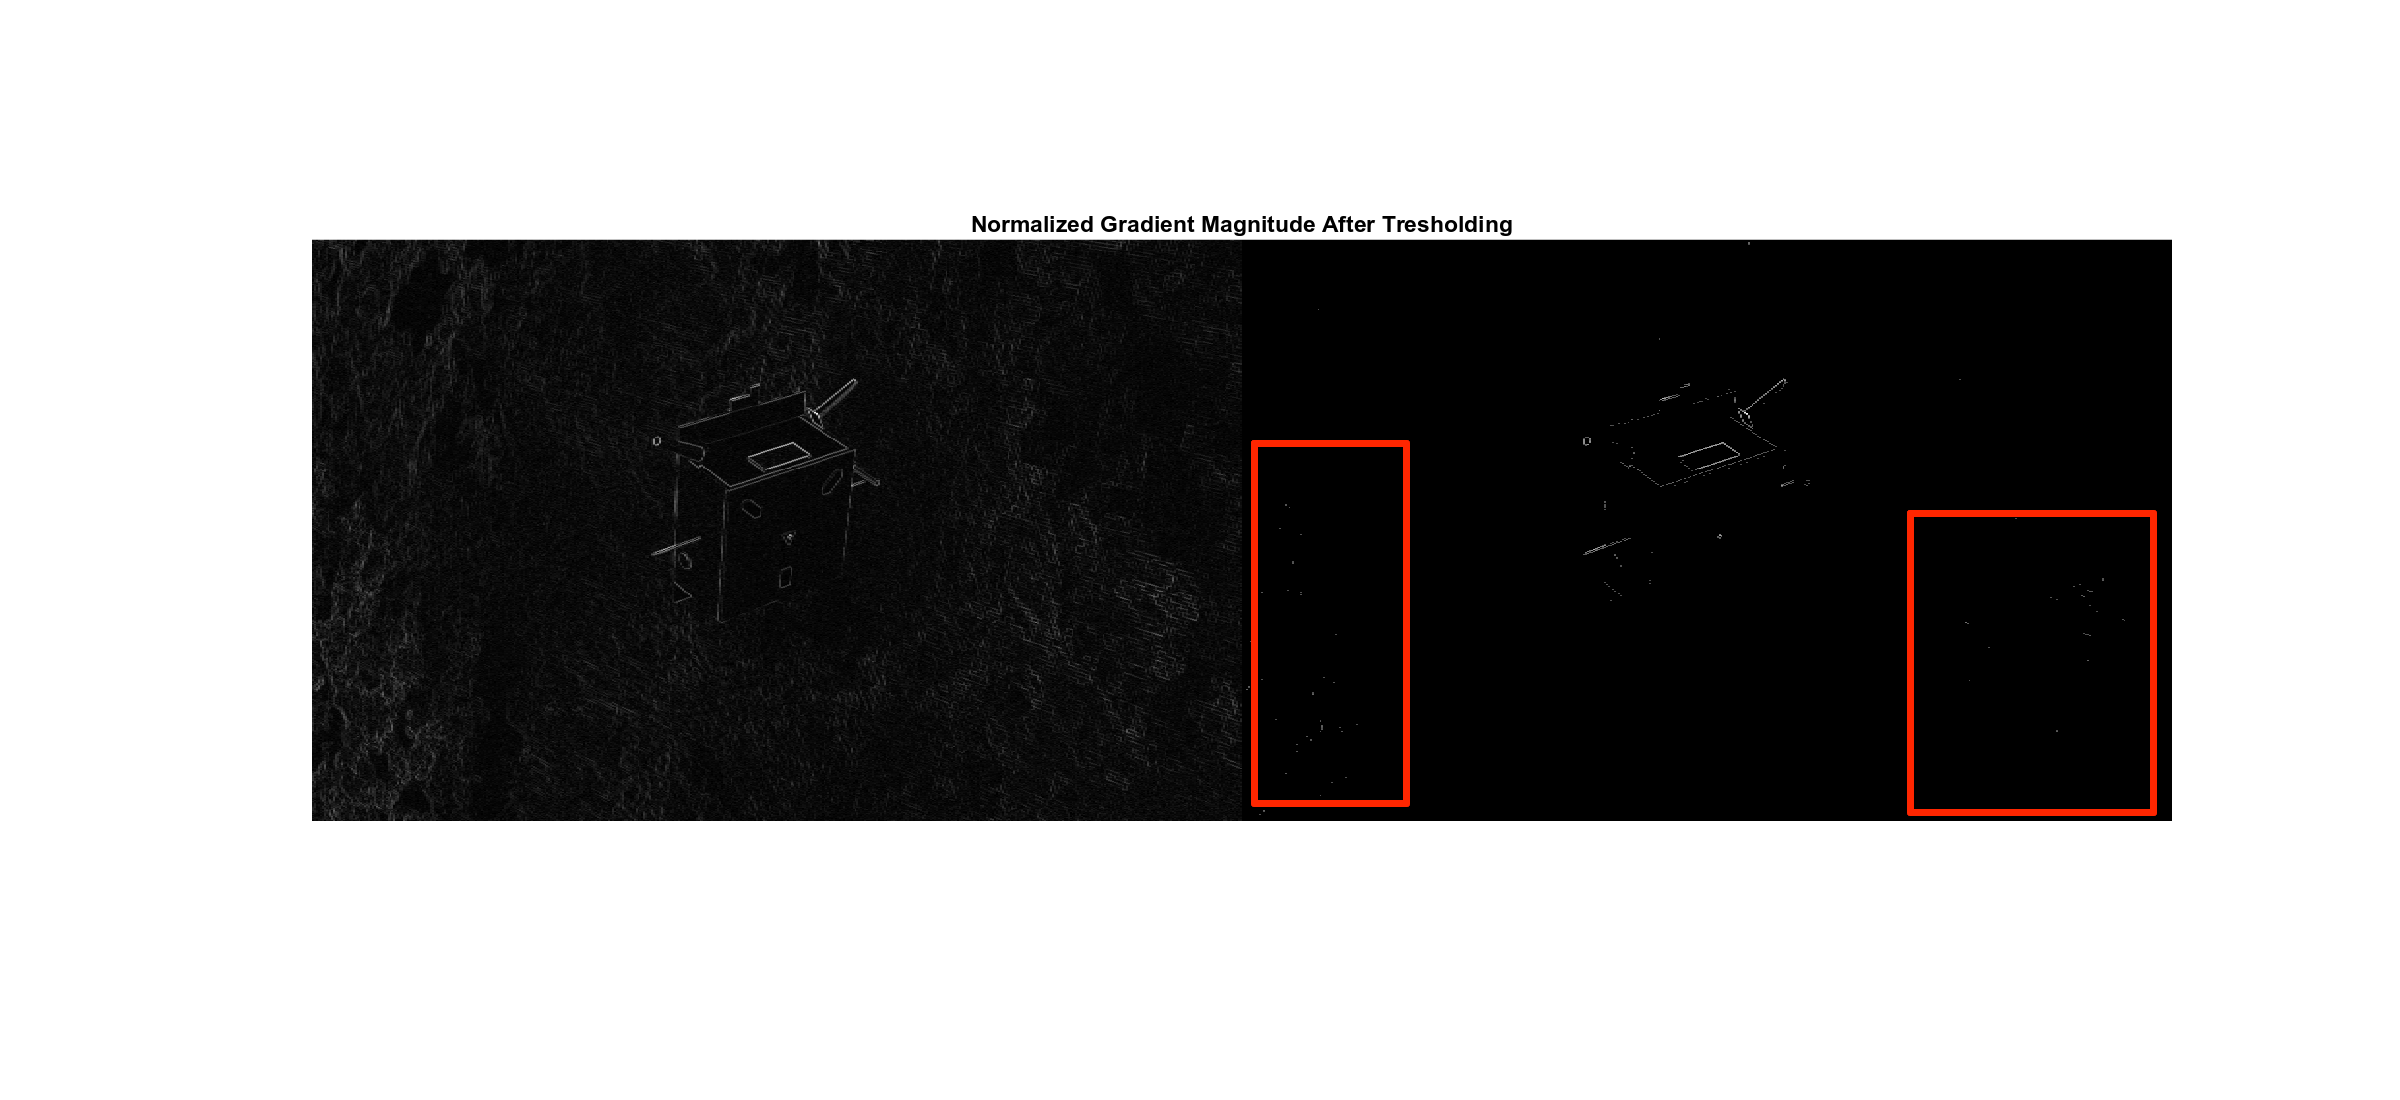
\includegraphics[width=1.0\textwidth]{gfx/results/prisma/117/8Select.png}
  \caption{Gradient image of figure \ref{fig:roiResults1}h}
\end{figure}

\begin{figure}[htbp]
  \centering
  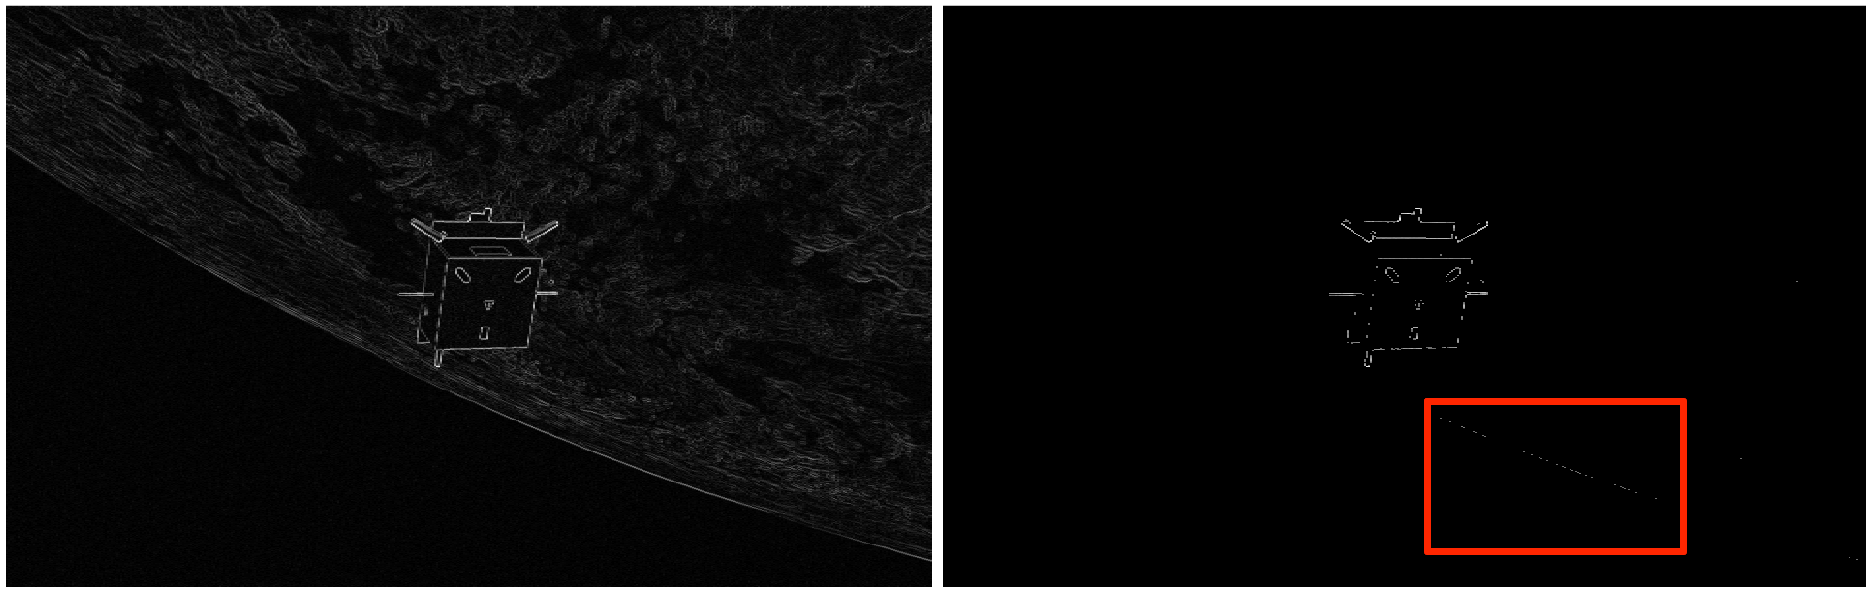
\includegraphics[width=1.0\textwidth]{gfx/results/prisma/164/8Select.png}
  \caption{Gradient image of figure \ref{fig:roiResults2}e}
\end{figure}

Moreover, the failure in the detection of the \acrshort{roi}, also also involves
the impossibility of rejecting spurious lines which do not belong to the silhouette of the \acrshort{sc} (as can be observed in figures \ref{fig:edgeDetection101}, \ref{fig:edgeDetection117} and \ref{fig:edgeDetection164}), and which would have been rejected in the case of a correct \acrshort{roi} selection.

\begin{figure}[htbp]
  \centering
  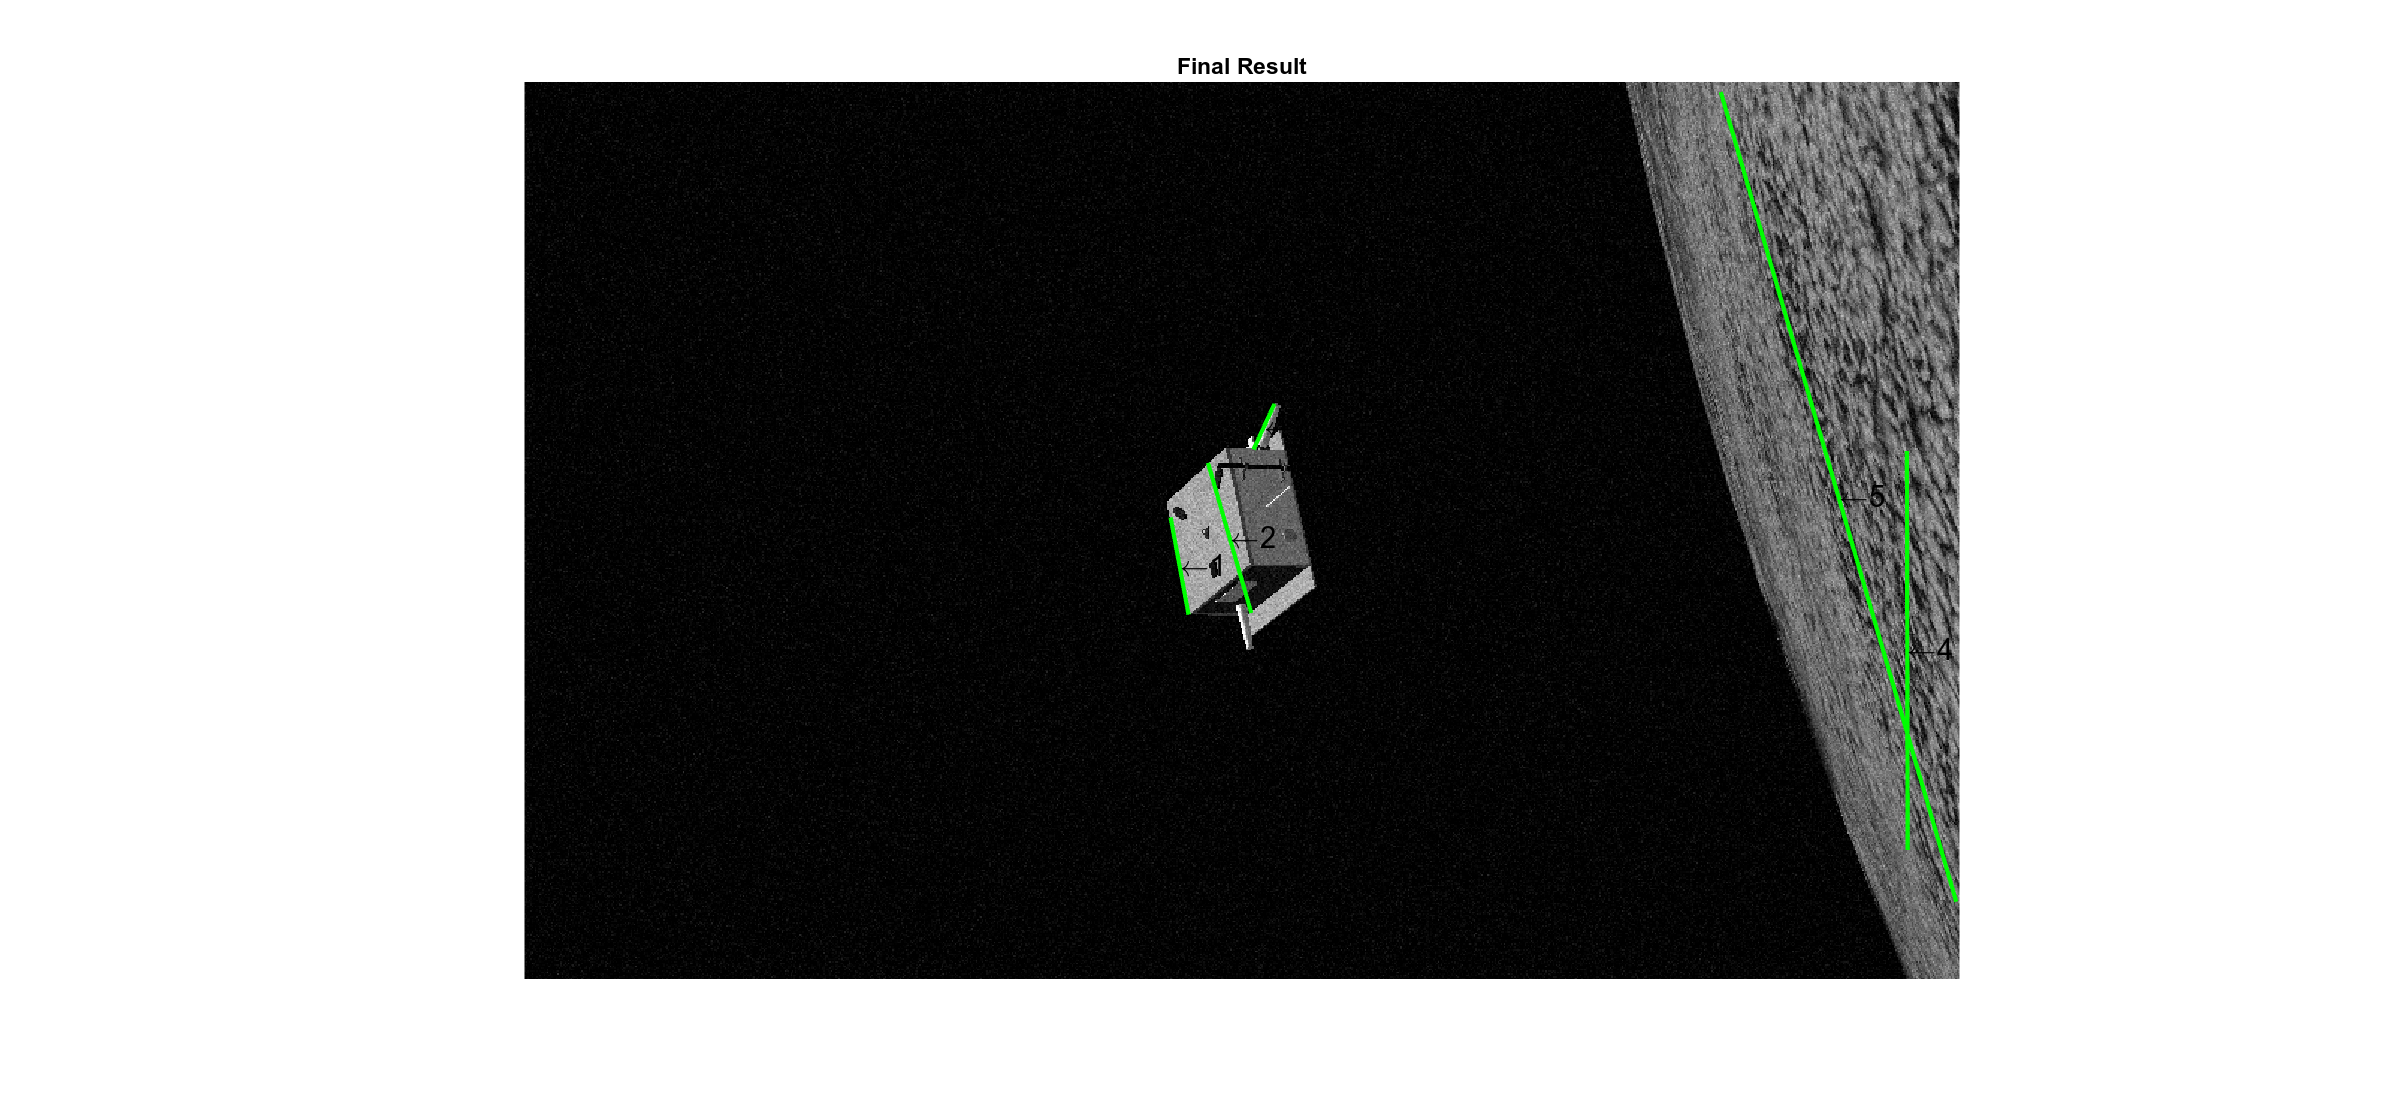
\includegraphics[width=1.0\textwidth]{gfx/results/prisma/101/15.png}
  \caption{Edge detection on figure \ref{fig:roiResults1}a}
  \label{fig:edgeDetection101}
\end{figure}

\begin{figure}[htbp]
  \centering
  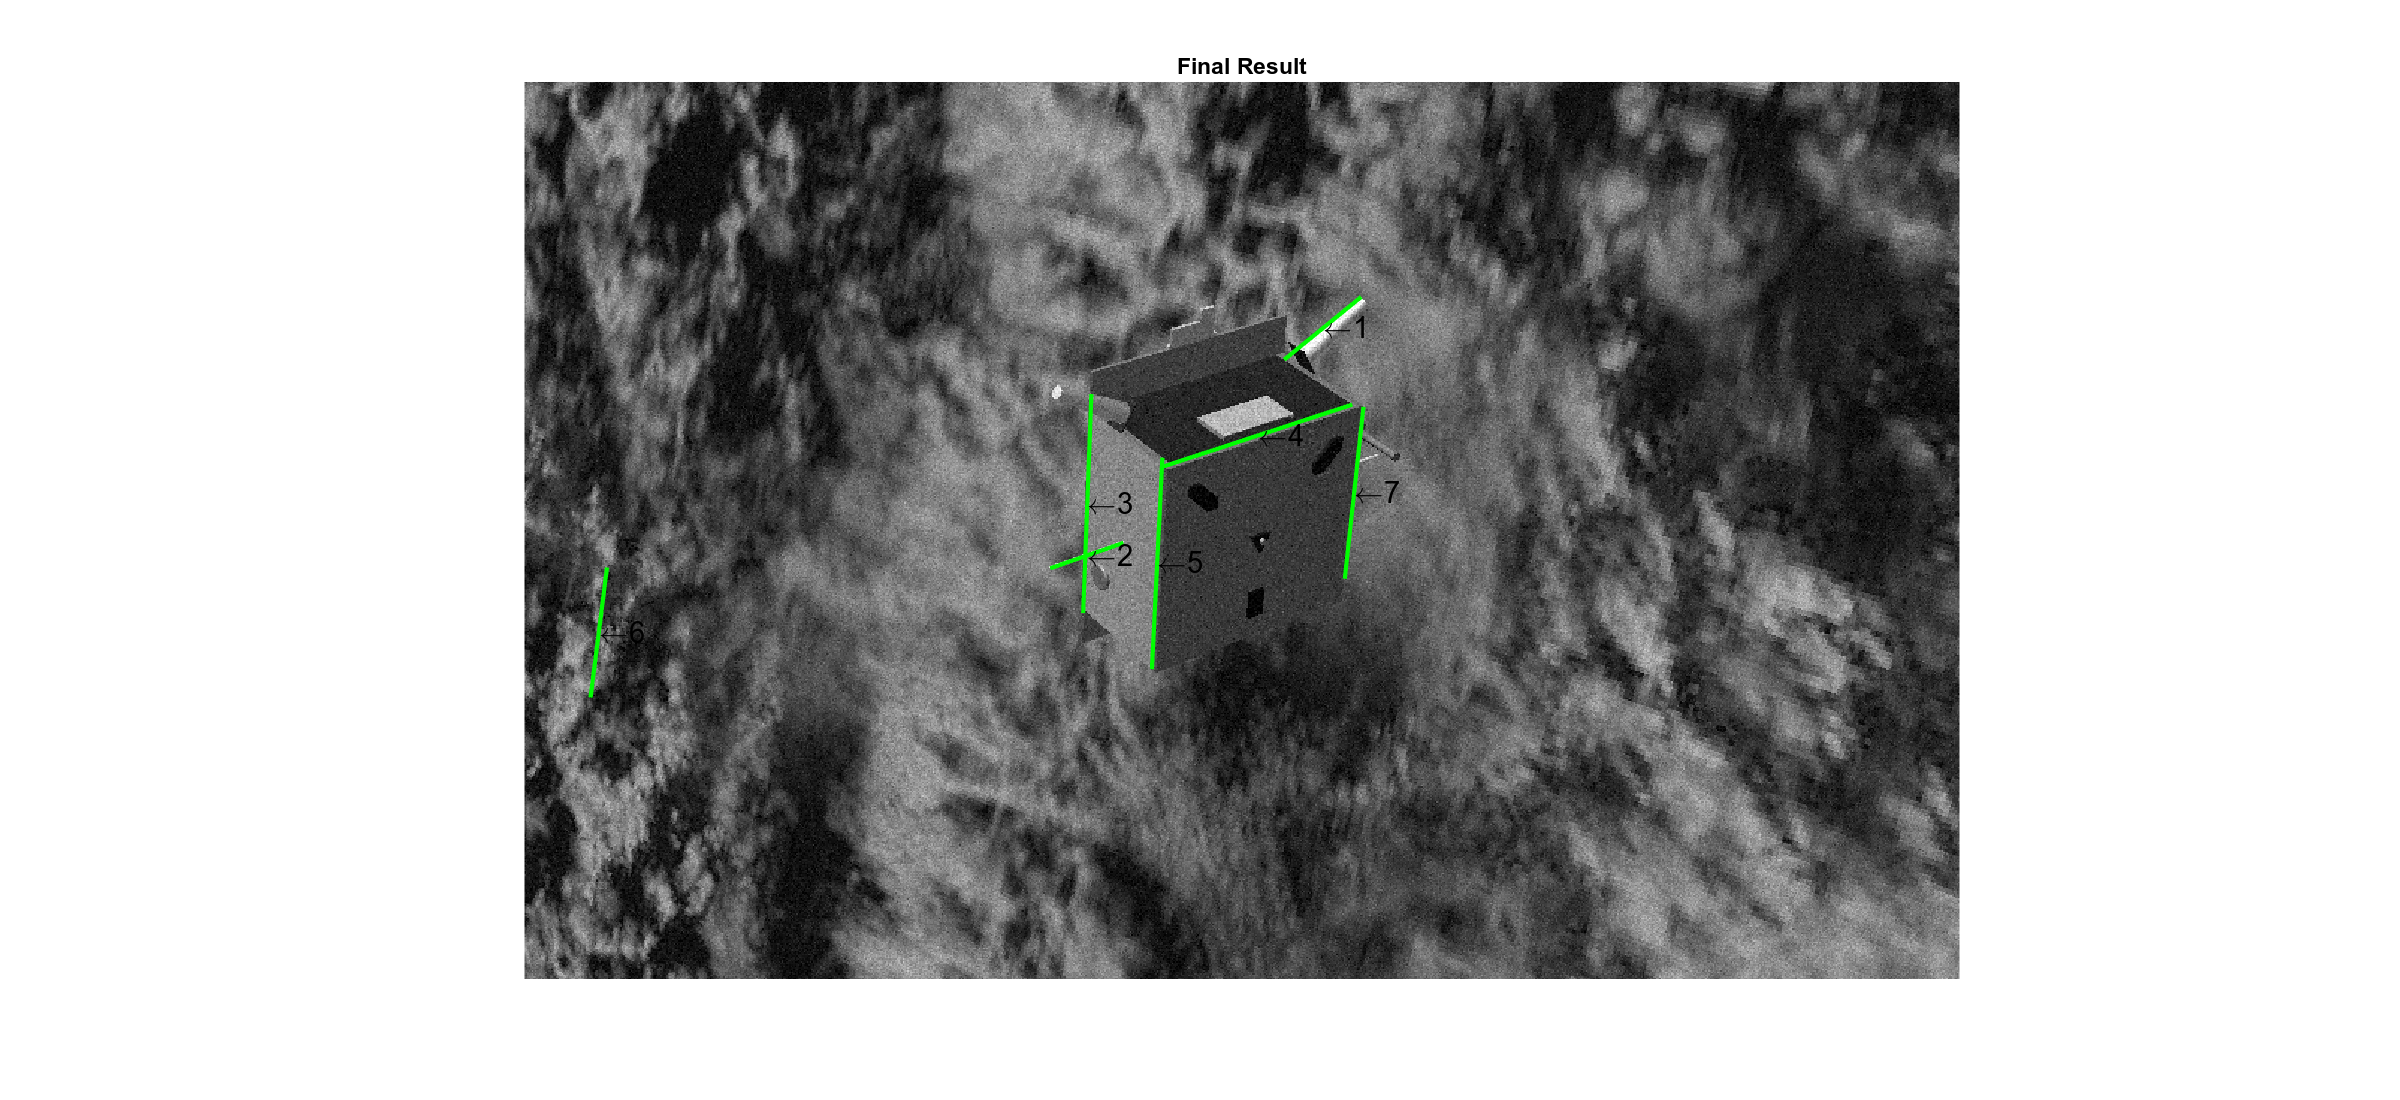
\includegraphics[width=1.0\textwidth]{gfx/results/prisma/117/15.png}
  \caption{Edge detection on figure \ref{fig:roiResults1}h}
  \label{fig:edgeDetection117}
\end{figure}

\begin{figure}[htbp]
  \centering
  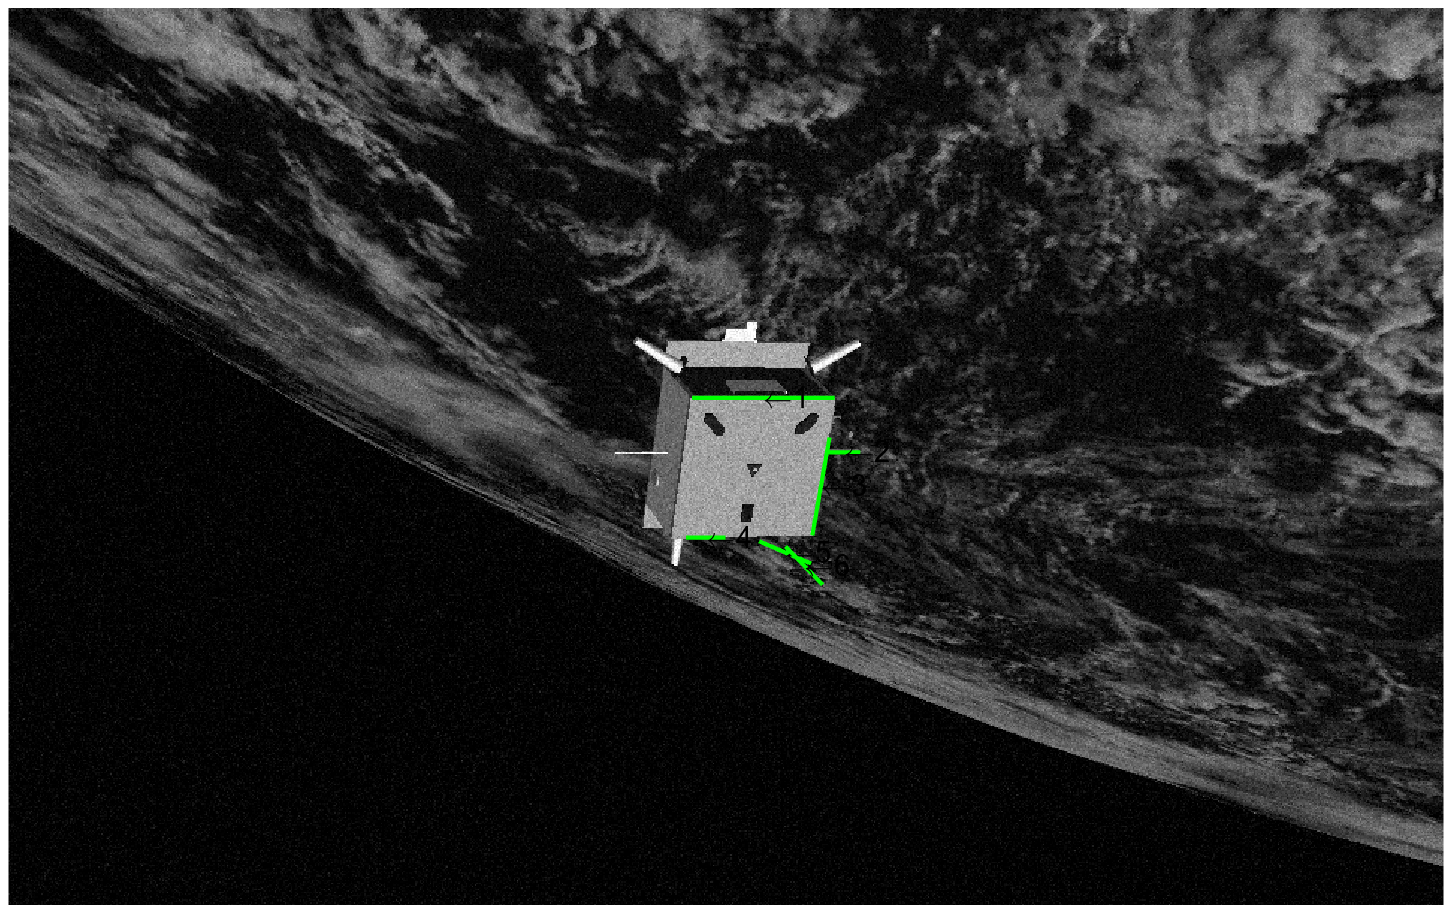
\includegraphics[width=1.0\textwidth]{gfx/results/prisma/164/15.png}
  \caption{Edge detection on figure \ref{fig:roiResults2}e}
  \label{fig:edgeDetection164}
\end{figure}

On one hand, one could think to increase more the filtering depth of the image, but on the other hand this will penalize too much the analysis of images which do not have a composite background.
As previously explained, a failure into the detection of the \acrshort{roi} greatly affects the performances of the \acrshort{svd} algorithm, since all the quantities which are computed as multiplicative constants of the \acrshort{roi} diagonal length will be biased.
For what concerns the edge detection procedure instead, as observed in \cite{Sharma2018}, further improvements must be made because it is still susceptible to producing spurious edges. Despite this being bad from the point of view of the \acrshort{cv} algorithm, this is good for what concerns the goodness of the generated data-set, which can reproduce more or less the same kinds of issues which the SPEED data-set had. In particular, it has been observed during this work that the most critical images are the ones where the solar panels are clearly visible and when the target \acrshort{sc} is far from the camera.
For what concerns the former case, it is particularly evident from figure \ref{fig:edgeDetection204}b that the culprit is likely due to the Sobel edge detector.

\begin{figure}[htbp]
  \centering
  \subfloat[]{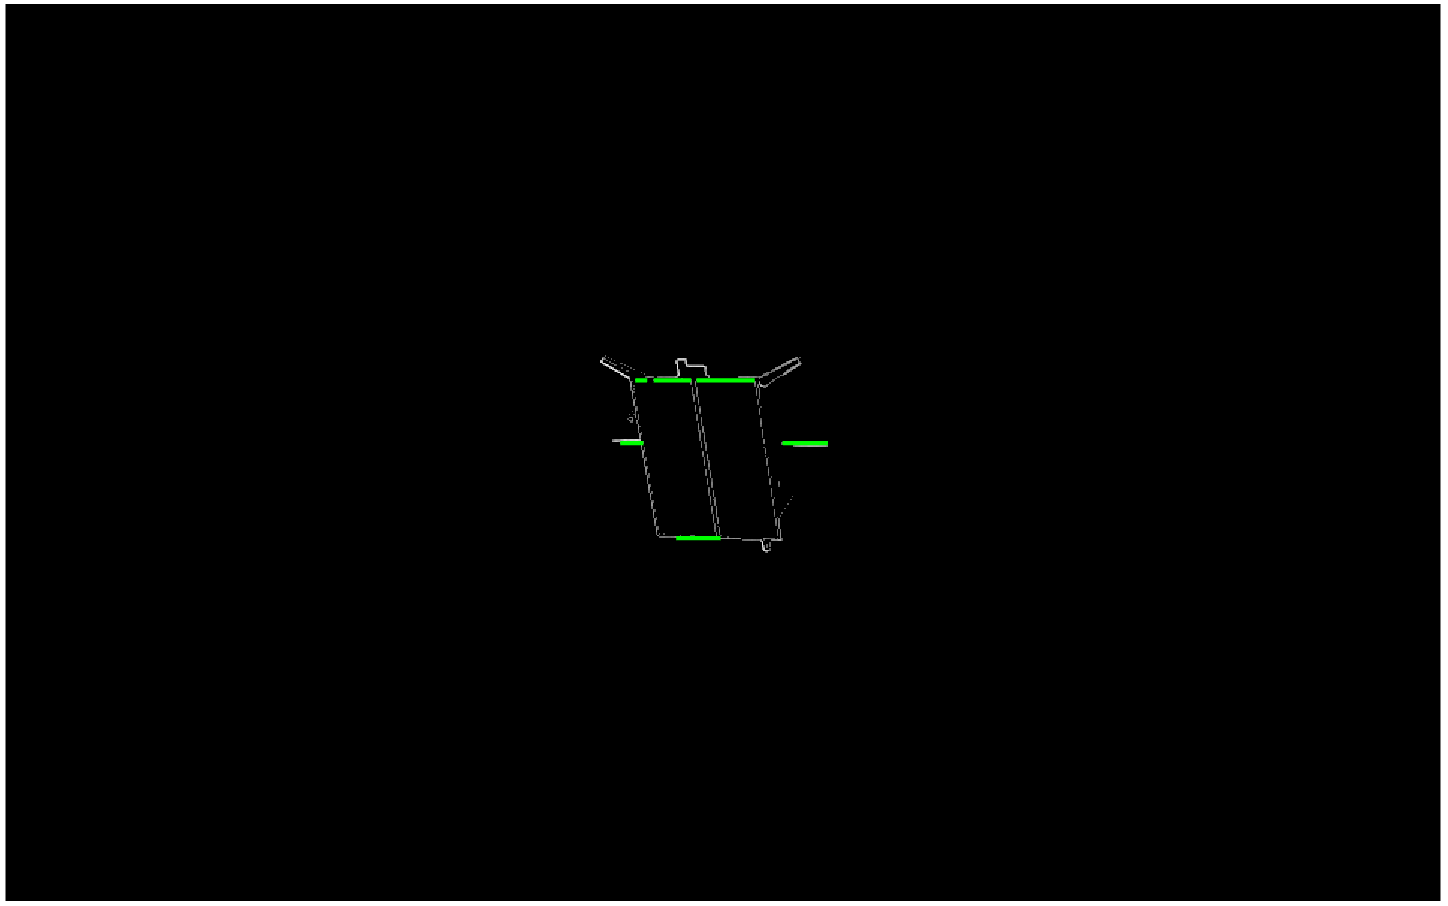
\includegraphics[width=0.45\textwidth]{gfx/results/prisma/204/10.png}}
  \qquad
  \subfloat[]{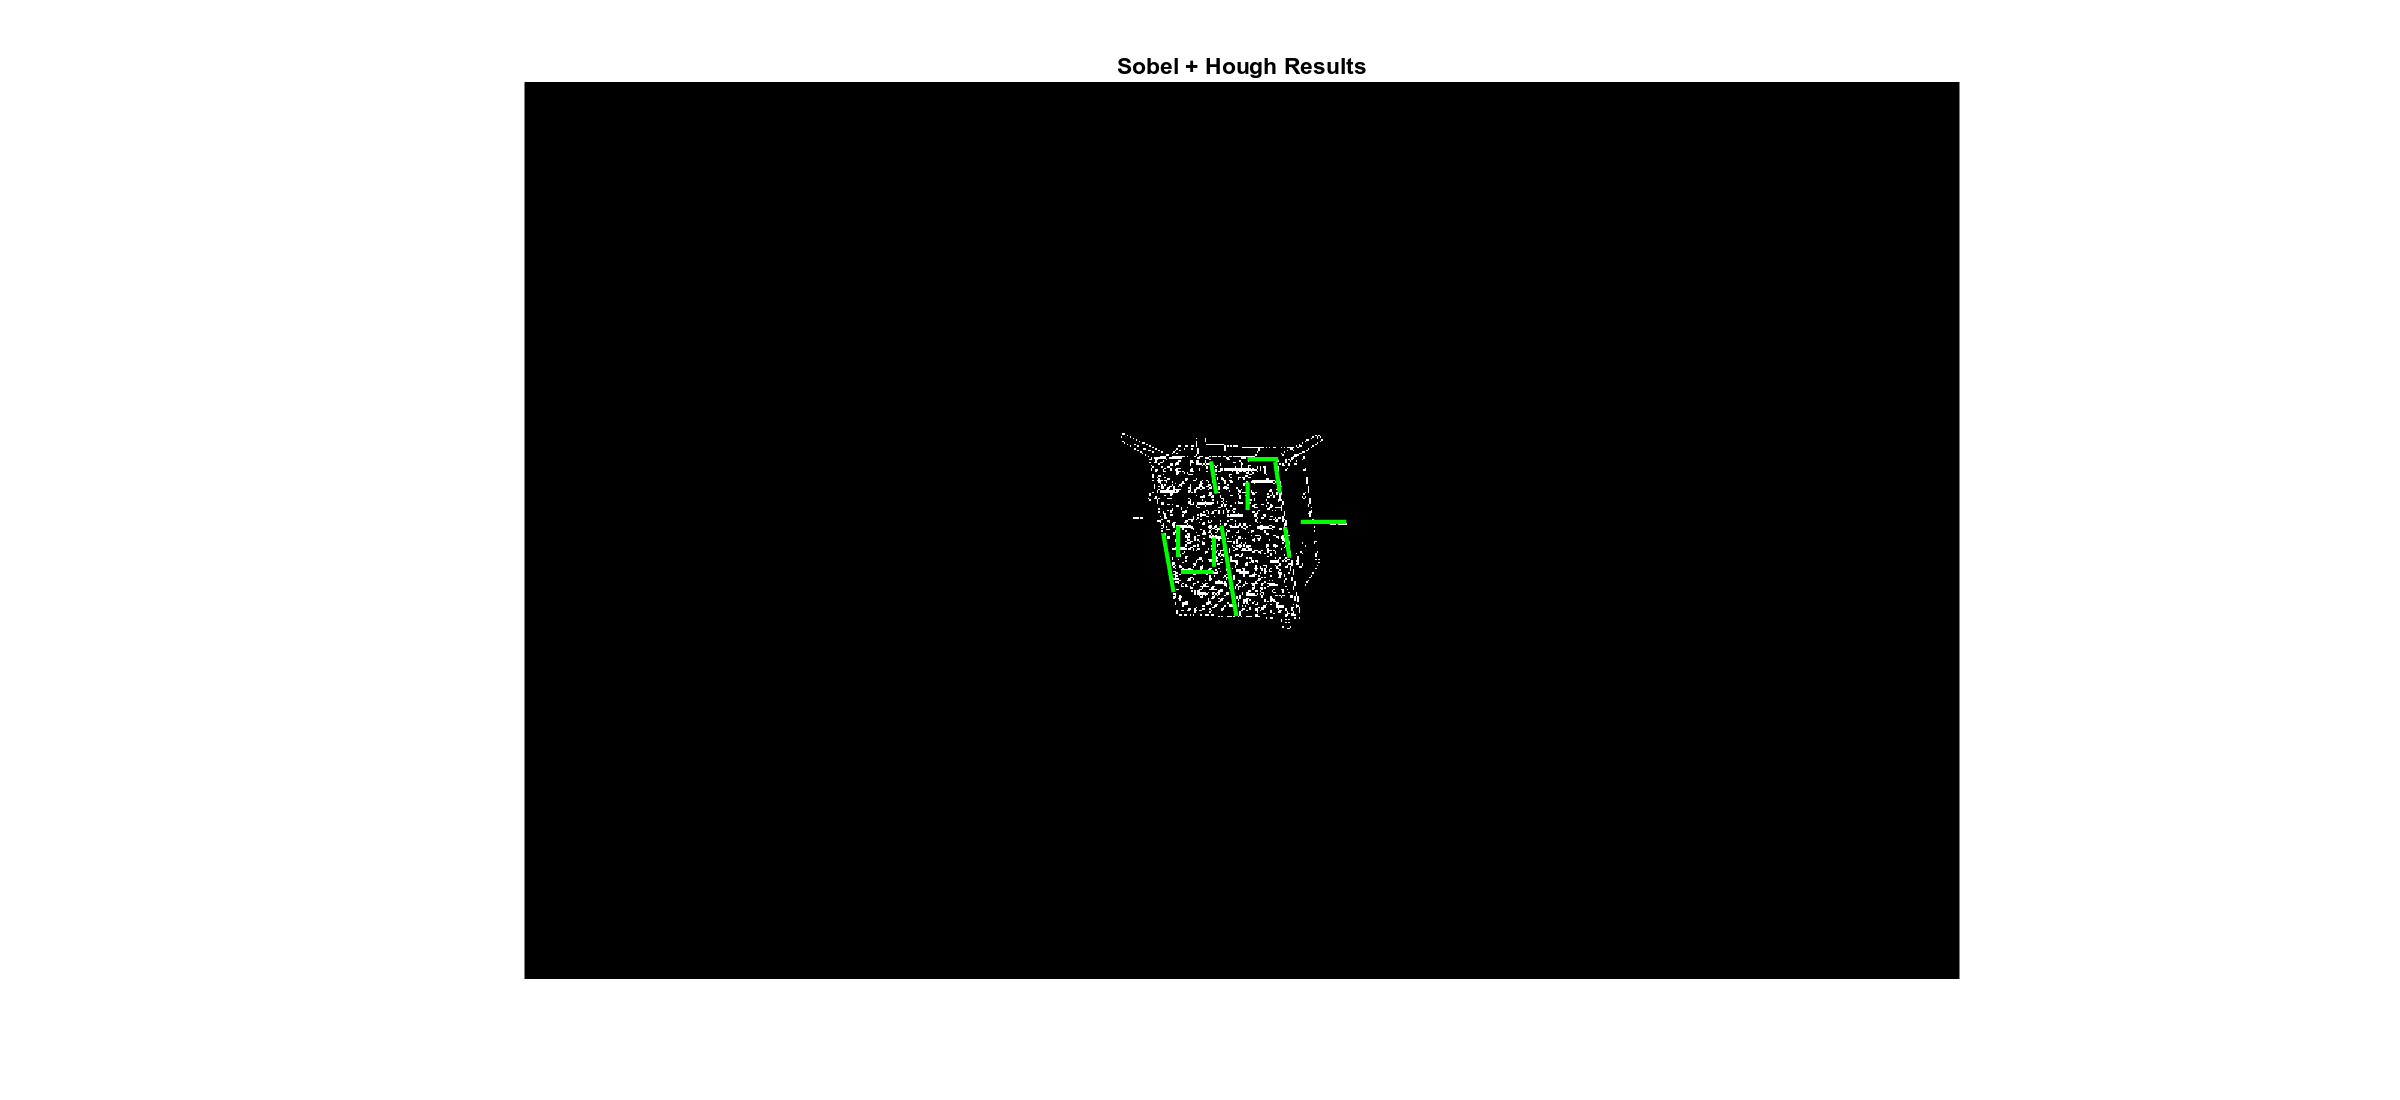
\includegraphics[width=0.45\textwidth]{gfx/results/prisma/204/11.png}}
  \qquad
  \subfloat[]{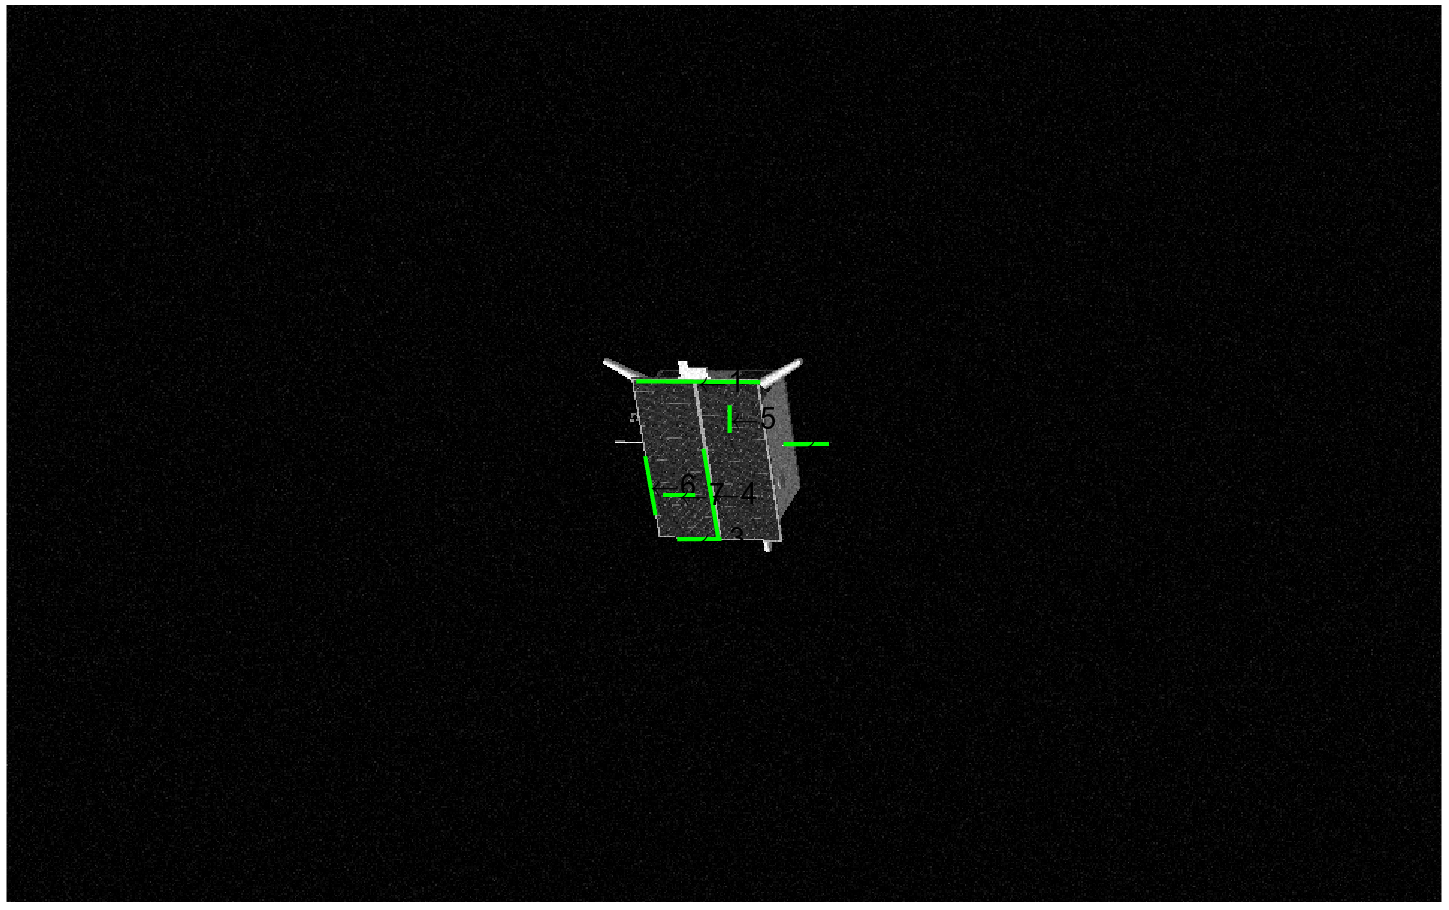
\includegraphics[width=0.45\textwidth]{gfx/results/prisma/204/15.png}}
  \qquad
  \caption{Image where the image processing subsystem contained spurious edges}
  \label{fig:edgeDetection204}
\end{figure}

While all the spurious points are filtered during by the \acrshort{wge} stream, they are not in the Sobel stream. Subsequently, when applying the Hough transform some spurious edge are detected. During the work on this project, some efforts have been made to cope with this issue which however has not been completely resolved, from what can bee seen in figure \ref{fig:edgeDetection204}c. On one hand, more treshold could be inserted into the image processing subsystem to take into account the presence of short spurious line and and remove them. On the other hand however, is really hard to fine tune those treshold in order to not remove other short edges which instead are useful, such as antennas.
There are also some particular attitudes where the Hough transform fails on the \acrshort{wge} filtered image, like for example what can be observed from figure \ref{fig:edgeDetection82}. In that case the ground truth relative pose was

\begin{equation*}
  \mathbf{A_{TC}} = \begin{bmatrix}
    0.8160 & -0.2675 & 0.5120 \\
    -0.5348        & -0.6850 & 0.4943 \\
    0.2183         & -0.6776 & -0.7021
  \end{bmatrix} \,,
\end{equation*}

\begin{equation*}
\mathbf{t_C} = [-3.60654 11.19394 11.59979] \ m \,.
\end{equation*}

\begin{figure}[htbp]
  \centering
  \subfloat[]{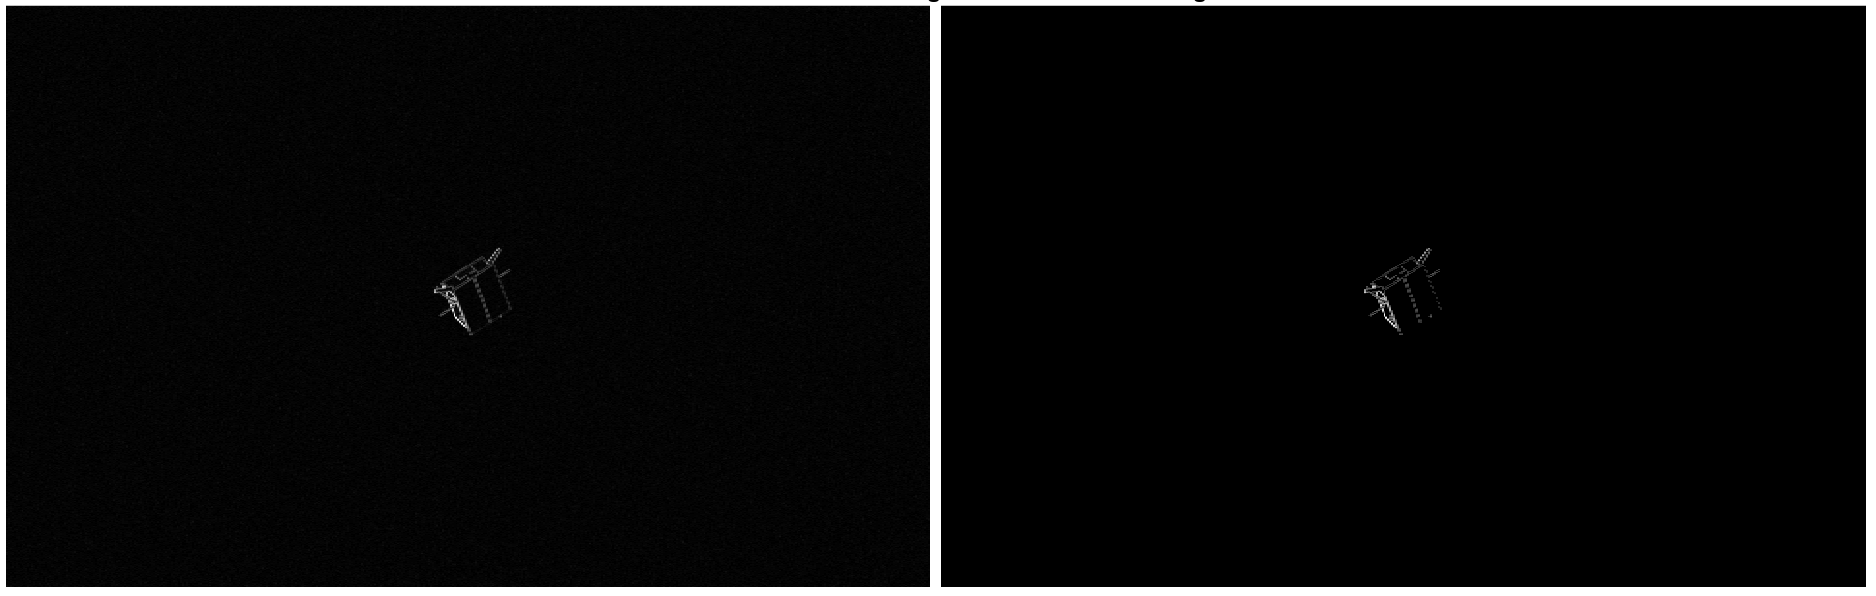
\includegraphics[width=0.45\textwidth]{gfx/results/prisma/82/8.png}}
  \qquad
  \subfloat[]{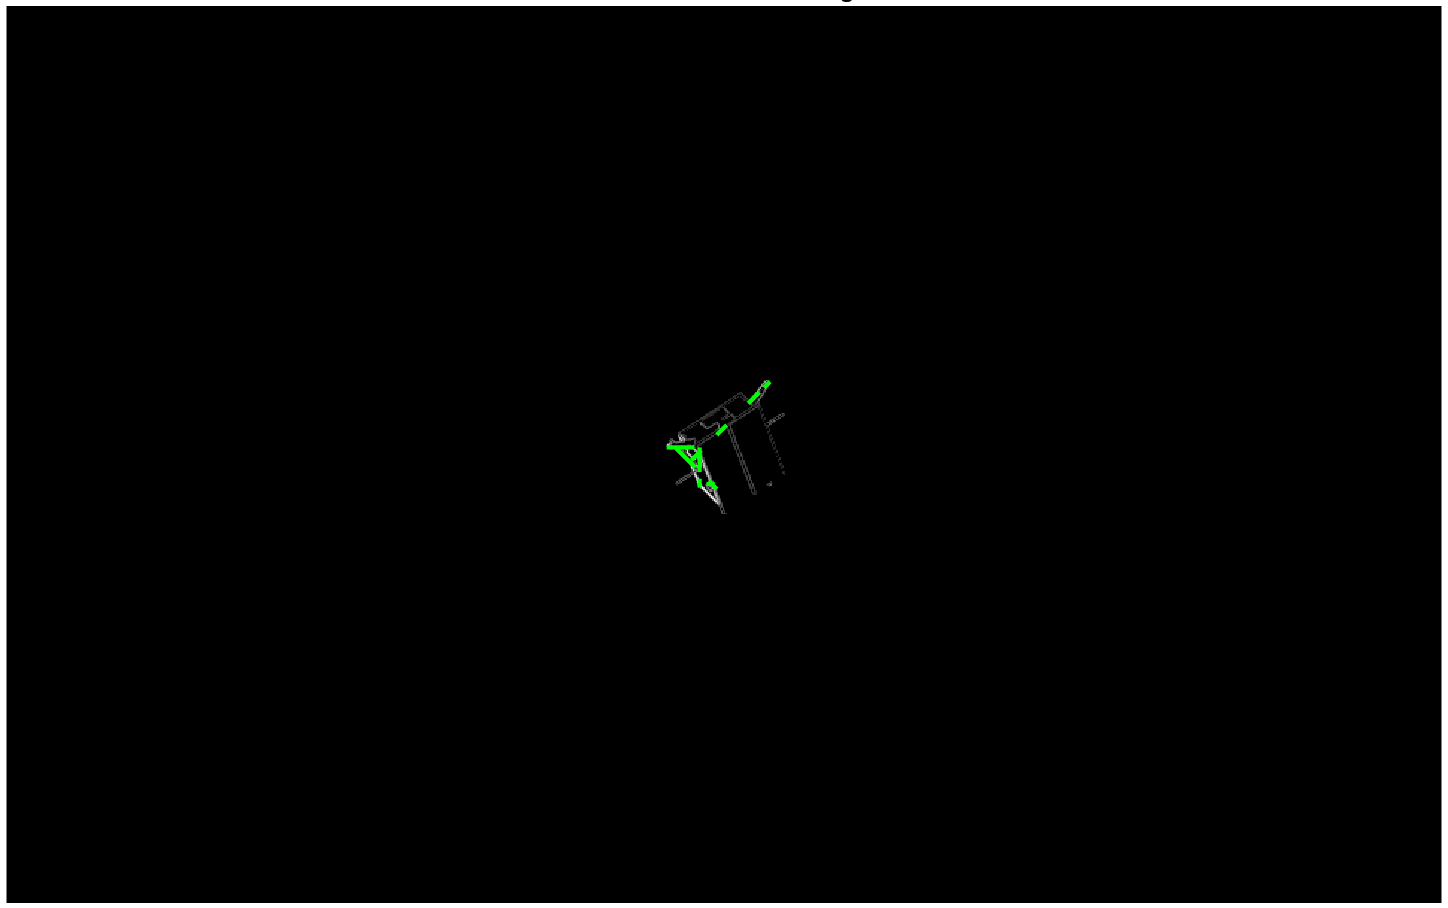
\includegraphics[width=0.45\textwidth]{gfx/results/prisma/82/10.png}}
  \qquad
  \subfloat[]{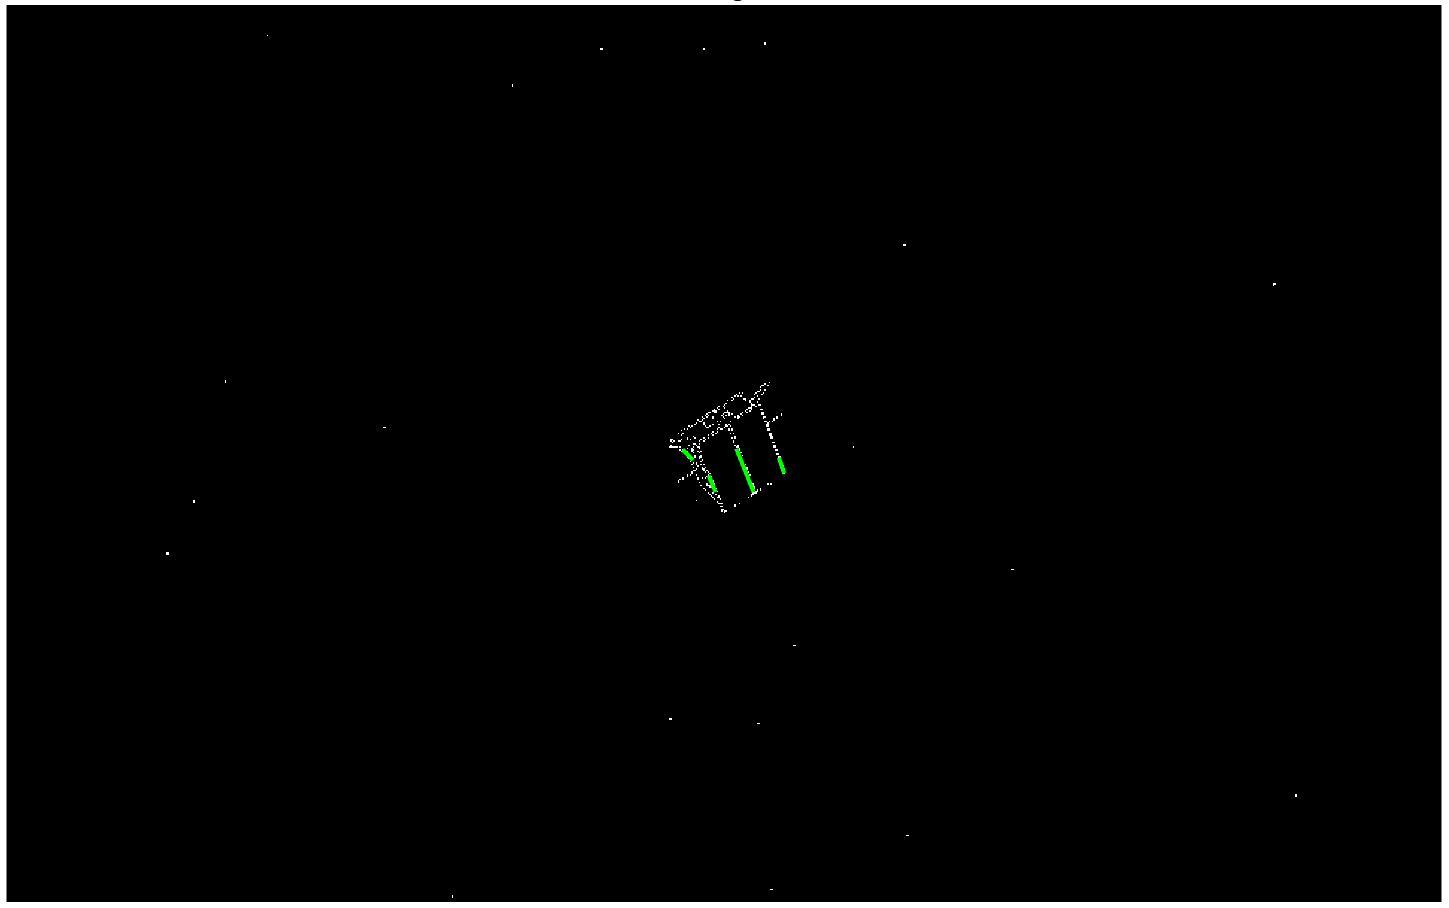
\includegraphics[width=0.45\textwidth]{gfx/results/prisma/82/11.png}}
  \qquad
  \subfloat[]{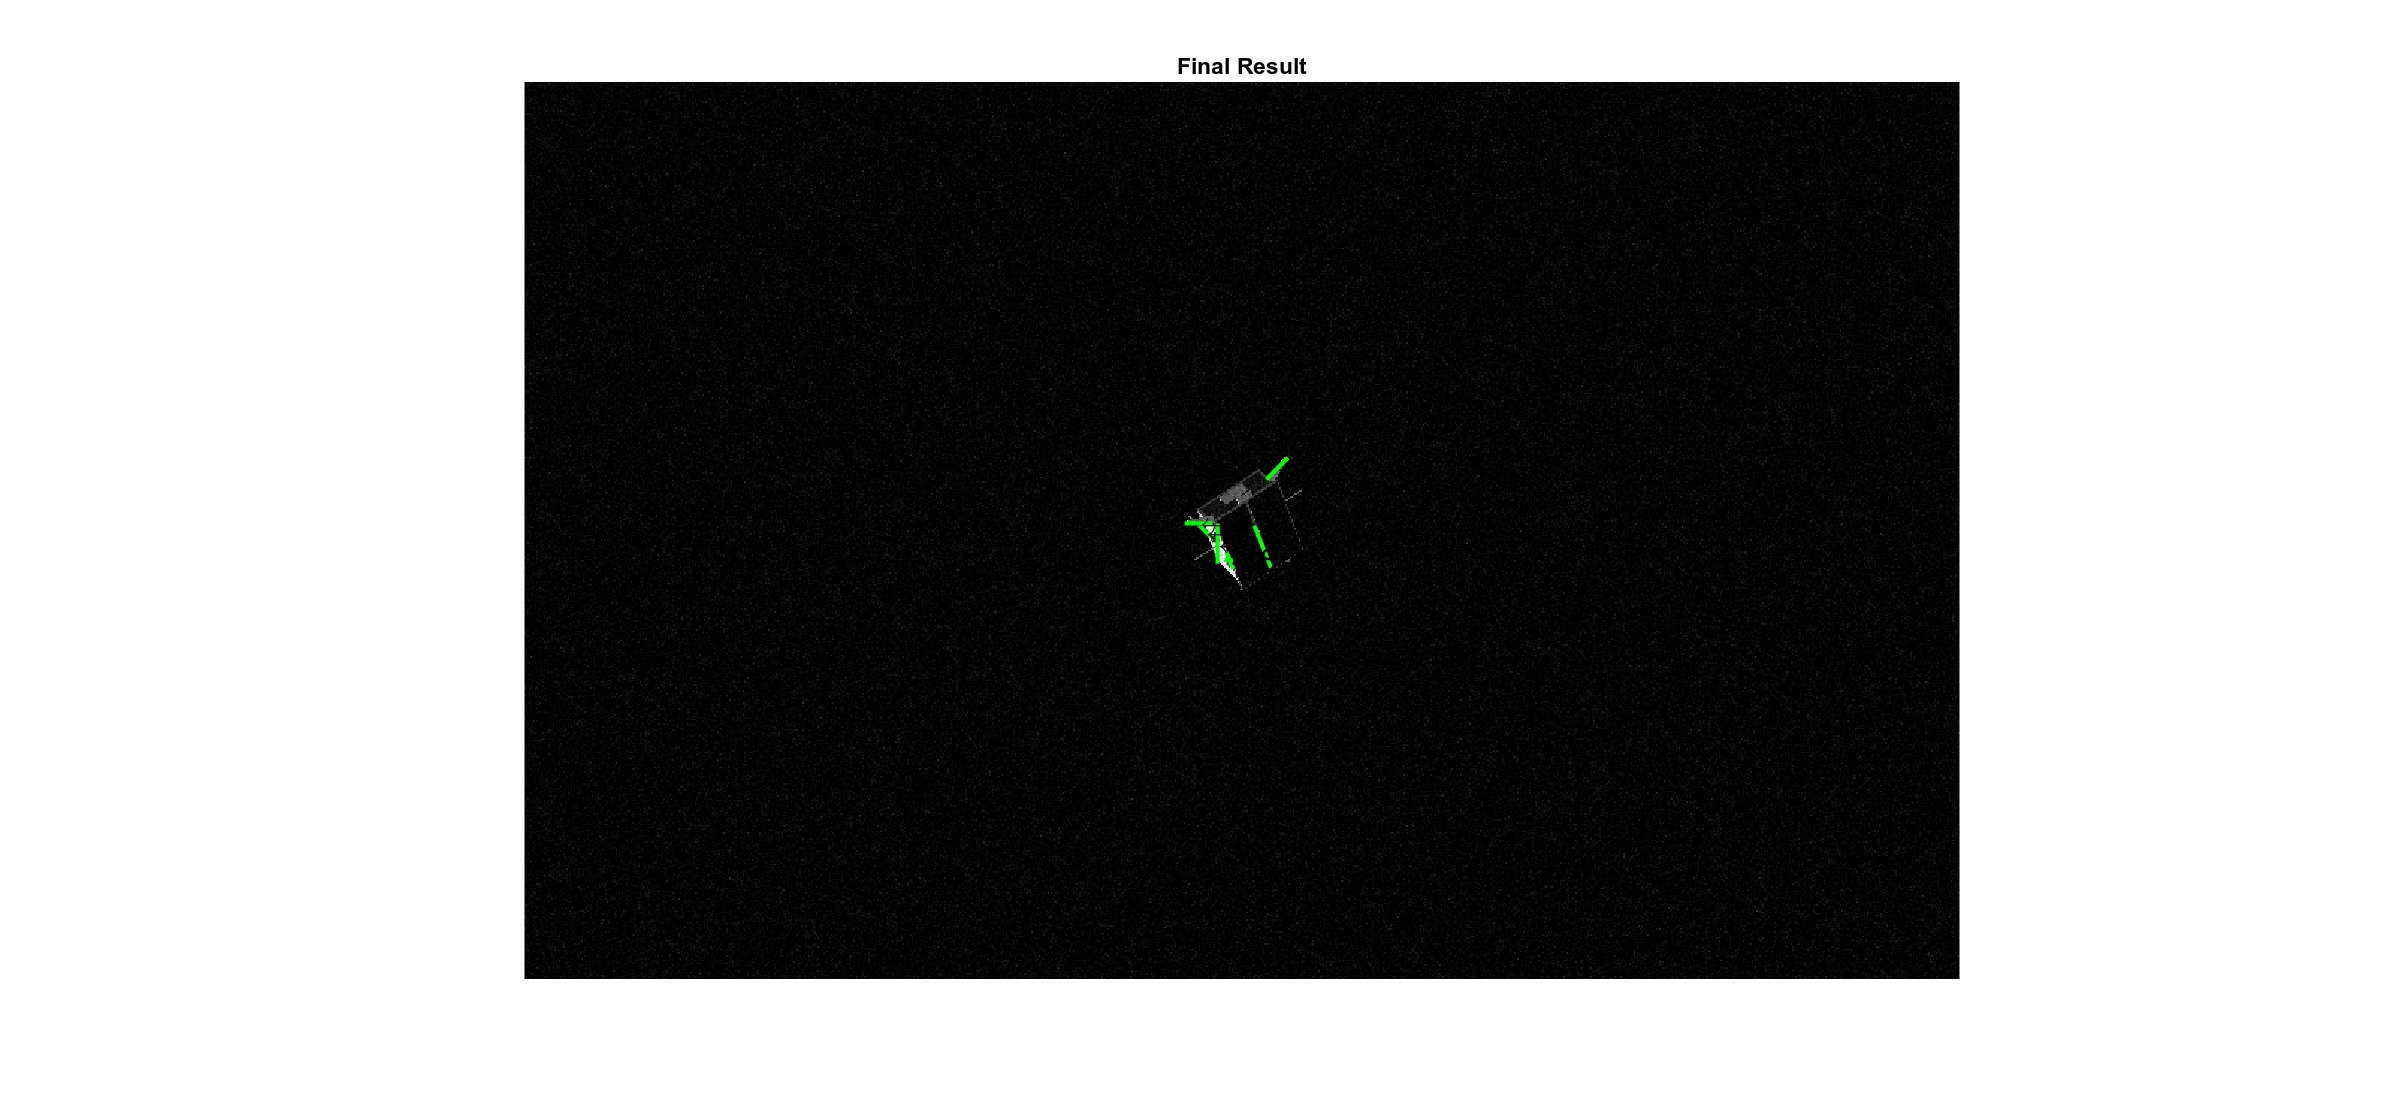
\includegraphics[width=0.45\textwidth]{gfx/results/prisma/82/15.png}}
  \qquad
  \caption{Image where the image processing subsystem contained not correctly detected edges}
  \label{fig:edgeDetection82}
\end{figure}

That result is likely to be due to the fact that the initial blur done to in order to filter out noise makes edges of the \acrshort{sc} harder to distinguish for the Hough transform if the target is relatively far from the camera, especially for some particular attitudes like the one shown. The result is that the algorithm results will loose accuracy as the relative distance grows.

When a perfect match is give to the pose estimator the mean error are *FARE SIMULAZIONE*